\section{The Fully Dynamic kNN Join}\label{sec:fdknnj}

In this section, we present the overall framework of our method, followed by the introduction of the dual-index schema designed for efficient computation, and finally, our cluster-based optimization for batch updates.

\subsection{Overview}\label{subsec:general analysis}

Given a query set $U$ and an answer set $I$ of $D-$dimensional, and an integer $k\leq|I|$, we present the overview of our framework for \fdknnj.
%
Firstly, the \emph{initial results} of the kNN Join, namely $kNN_{\bowtie}(U,I)$, are computed.
%
We discuss the process for each type of updates in $U$ or $I$ as follows.


\stitle{Case 1 - Insertion into $\mathbf{I}$:}
%
When a data point $q$ is inserted into the answer set $I$, namely $I'=\oplus_I(q)$, an RkNN search $RkNN(q,U,I')$ is performed to identify all data points $u_i\in U$ whose results are affected by $q$, i.e., $\exists p\in kNN(u_i,I), dist(q,u_i)\leq dist(p, u_i)$\footnote{We choose to update the kNN of $u\in U$ to include $q$ if the distance between $q$ and $u$ equals the distance to $u$'s previous $k$-th nearest neighbor in $I$ to maintain result ``freshness''.}.
%
Then, for each $u_i$, its previous $k$-th nearest neighbour in $I$, namely $NN_k(q,I)$, is removed and replaced with the newly inserted $q$. 

\stitle{Case 2 - Deletion from $\mathbf{I}$:}
%
When a data point $q$ is deleted from the answer set $I$, namely $I'=\ominus_I(q)$, a RkNN search $RkNN(q,U,I)$ is performed to identify all data points $u_i\in U$ whose results will be affected by the deleted $q$, i.e., $q\in kNN(u_i,I)$.
%
Then, $kNN(u_i, I')$ is updated for each $u_i$.

\begin{remark}
It is worth noting that an alternative approach for Cases 1 and 2 is to recompute the kNN for each point in $U$ after the update.
%
However, this naive approach incurs significant time costs and redundant computation \cite{yang2014continuous,ukey2022efficient, yu2010high, ukey2023efficient}. 
%
The strategy of identifying affected data points in set $U$ through an RkNN search leads to reduced computation and much more efficient updates.
\end{remark}

\stitle{Case 3 - Insertion into $\mathbf{U}$:}
%
When a data point $u$ is inserted into the query set $U$, the algorithm computes $kNN(u,I)$ and adds the pair of $(u,kNN(u,I))$ to the result set.

\stitle{Case 4 - Deletion from $\mathbf{U}$:}
%
When a data point $u$ is deleted from the query set $U$, the algorithm deletes the data point $u$ with its associated $kNN(u,I)$ from the result set.

\begin{remark}
    Case 4 is considered a trivial operation; hence, further discussion on this type of updates is omitted in the rest of the paper.
\end{remark}

Next, we will introduce the dual-index structure designed for handling above updates and the cluster-based optimization for efficient batch updates.


\subsection{Dual-Index Structure}

 
In \fdknnj, as described above, two of the most time-consuming operations are RkNN search (in Cases 1 and 2) and kNN search (in Cases 2 and 3). A common technique to speed up such operations is building index structures \cite{lin1994tv, ciaccia1997m, yu2001indexing, bohm2004k, xia2004gorder, jagadish2005idistance, yu2007efficient, yu2010high, yang2014continuous}.
%
However, existing methods are mainly designed for partially dynamic kNN join, and they usually adopt a \emph{single-index} schema in indexing.
%
For example, the \hdrtree proposed in \cite{yang2014continuous} is a single tree constructed on the query set $U$. It supports efficient RkNN Search on $U$ for the updated points in $I$. However, due to the lack of efficient support for kNN search, it can be inefficient when we are deleting from $I$ (Case 2) and inserting into $U$ (Case 3).
%
Considering the scenario where only an \hdrtree is built on $U$ and $I$ contains $500,000$ data points, determining the k-nearest neighbors for one new point in $U$ requires a minimum of $500,000$ distance computations on full dimensions. This translates to over $25$ billion distance calculations on full dimensions if $50,000$ points are inserted into $U$.

Conversely, relying on a single index structure built on $I$ cannot facilitate an efficient RkNN Search, leading to a high computational load to process Cases 1 and 2.

To address the limitations of a single-index structure, we propose to employing a \emph{dual-index} structure built on both $U$ and $I$ to enable both efficient kNN and RkNN processes in \fdknnj. 


Our dual-index structure, referred to as \dualtree, consists of an \hdrtree \cite{yang2014continuous} for the query set $U$ and a \deltatree \cite{cui2003contorting} for the answer set $I$, with essential updates to support \fdknnj.
%
The \hdrtree has demonstrated superior performance in recent works on partially dynamic kNN join \cite{ukey2022efficient,ukey2023efficient,ukey2023survey,ukey2023knn}. We leverage it to help with the RkNN search in insertion and deletion of data points within $I$ in \fdknnj.
%
\deltatree, on the other hand, enables efficient kNN search for newly inserted data points in the query set $U$ and has proven to be powerful for high-dimensional kNN search compared to other existing methods such as TV-Tree \cite{lin1994tv}, M-Tree \cite{ciaccia1997m}, VA-file \cite{weber1998quantitative}, i-distance \cite{yu2001indexing}, and CR-Tree \cite{kim2001optimizing}.
%
Moreover, when data points are deleted from the answer set $I$, the \deltatree enables fast re-computation of the kNN results for the $u_i\in U$ whose results are affected by the deleted points.
%
Both \hdrtree and \deltatree apply PCA as the dimensionality reduction technique and use hierarchical clustering to effectively index high-dimensional data in tree structures, as will be introduced later.


Given that both $U$ and $I$ are dynamically updated in \fdknnj, the \hdrtree built on $U$ and the \deltatree built on $I$ within our \dualtree structure need to be updated accordingly.
%
While \deltatree natively supports updates \cite{cui2003contorting}, \hdrtree is originally designed for static data, i.e., the query set in partially dynamic kNN join is static, and therefore does not support updates.
%
To address this issue, we also propose the algorithms for updating the \hdrtree.
In the following content, we will discuss the concrete structure and the construction strategy of the dual-index structure. 


\stitle{Structure of \bdualtree.}
%
A \dualtree consists of a \hdrtree and a \deltatree, each with its own parameters.
%
They are denoted as $f_\text{HDR}$ and $t_\text{HDR}$ for the \hdrtree, and $f_\Delta$ and $t_\Delta$ for the \deltatree. 
%
Here, $f_\text{HDR}$ and $f_\Delta$ represent the fanout, while $t_\text{HDR}$ and $t_\Delta$ represent the threshold of node size for the respective trees.
%
Example trees are illustrated in Fig. \ref{fig:cluster_based_update} with $f_\text{HDR}=f_\Delta=2$.

\sstitle{\hdrtree.}
%
In the \dualtree schema, the \hdrtree is constructed on the query set $U$. Each node in the \hdrtree can be a \textit{leaf} node or a \textit{non-leaf} node. For a leaf node, it directly contains points assigned to it. For a non-leaf node, it consists of $f_\text{HDR}$ clusters of data points in the reduced PC space, and each child of the node further divides the data in a cluster.
%
The node will not be further divided if the number of data points assigned to it is smaller than $t_\text{HDR}$, i.e., the leaf nodes.
%
The estimated height $L_\text{HDR}$ of the \hdrtree is $log_{f_\text{HDR}}(|U|)$.
%
Each level $l$ of the \hdrtree corresponds to a PC space with a distinct number of dimensions $d_\text{HDR}(l) \leq D$, decided by 

\begin{flalign}
    d_\text{HDR}(l)=min\{d | \frac{\sum_{i=1}^{d}\sigma_{M_{PC}}^U(i)}{\sum_{i=1}^{D}\sigma_{M_{PC}}^{U}(i)}\geq \frac{l}{L_\text{HDR}}\}      \IEEEyesnumber \label{eq: level_decision}
\end{flalign}

\noindent where $M_{PC}$ is initialized by the initial state of $U\cup I$. 
%
In other words, the proportion of the sum of variance of the points in $U$ for the first $d_\text{HDR}(l)$ dimensions in $M_{PC}$ over the total variance of the full $D$ dimensions should be no smaller than the proportion of $l$ over $L_\text{HDR}$.


For non-leaf nodes in the $d_\text{HDR}(l)$-dimensional PC space, as they are divided into $f_\text{HDR}$ clusters, the following properties are stored for each cluster $C^i_l$:
%
1) the data points assigned to it in the corresponding PC space;
%
2) its center in the PC space denoted as $center_{PC}(C^i_l)$, which is the projection in the $d_\text{HDR}(l)$-dimensional PC space of its center denoted as $center(C^i_l) = \sum_{v_j\in C^i_l} \frac{v_j}{|C^i_l|}$;
%
3) its radius in the $d_\text{HDR}(l)$-dimensional PC space, denoted as $radius_{PC}(C^i_l)=\max_{v_j\in C^i_l}dist_\text{PC}(center(C^i_l),v_j)$; 
%
4) the maximal value of the distances between its assigned points and their $k$-th nearest neighbors, denoted as $dist_\text{MkNN}(C^i_l)=\max_{v_j \in C^i_l}dist_\text{kNN}(v_j,I)$;
%
and 5) pointers to its corresponding child nodes.
% 
By utilizing the hierarchically structured and cluster-based design, \hdrtree can prune unpromising nodes in lower dimensions (i.e., lower levels of the tree) when performing an RkNN search, thereby improving its efficiency.


\sstitle{\deltatree}:
The \deltatree within the \dualtree is built on $I$. The design and structure of \deltatree are similar to those of \hdrtree. Due to space limitations, we omit the details here.
%
The major difference is that $dist_\text{MkNN}$ is not recorded for the clusters in \deltatree.
%
This is because \hdrtree is built on $U$, and $dist_\text{MkNN}$ is designed to prune unpromising candidates in an RkNN search in \fdknnj. However, \deltatree is built on $I$ to speed up kNN search, where the property of $dist_\text{MkNN}$ does not exist.


\stitle{Construction of \bdualtree.}
%
The construction of a \dualtree involves building both a \hdrtree and a \deltatree. Both trees follow the strategy of recursively splitting non-leaf nodes until the number of data points in a node reaches the threshold, i.e., $t_\text{HDR}$ or $t_\Delta$.
%
Following previous work \cite{cui2003contorting, yang2014continuous, ukey2022efficient, ukey2023efficient}, we utilize the $k$-means algorithm \cite{macqueen1967some,singh2013k} during clustering. The results of $KNN_{\bowtie}(U,I)$ for the initial state of $U$ and $I$ are computed in advance before construction.
%
%\todo{Due to space limitations, the details are omitted in this paper.}

\stitle{\bdualtree Maintenance.} 
%
In \fdknnj, both sets $U$ and $I$ are dynamically updated. Consequently, \dualtree also needs to support dynamic updates to maintain an up-to-date index. In the following, we discuss the maintenance on our \dualtree index in different cases.

\sstitle{Case 1 and Case 2.} 

When in Case 1 or Case 2 where data points are inserted into or deleted from $I$, in addition of the corresponding operation of the updated points in the \deltatree part of the \dualtree which is built on $I$, update is also needed for the \hdrtree part. Except for the influence on the spatial features of the data points in $I$ which requires update of the \deltatree part, there is also a possibility that update in $I$ affects the KNN Search results over $I$ of some data points in $U$, leading to the change of their $dist_{KNN}$ values. Observing that the \hdrtree part of the \dualtree is not only built on $U$ but also contains the feature related to $I$, that is the maximal value (i.e., $dist_{MkNN}$) of the $dist_{kNN}$ values of the data points in each of its cluster introduced for the pruning steps in RKNN Search, we also update the $dist_{MkNN}$ values of the \hdrtree part of the \dualtree when update in $I$ to ensure correct and efficient RKNN Search.

In conclusion, when update in $U$ and $I$, both the \hdrtree and the \deltatree part of the \dualtree need to be updated. Especially when update in $I$, not only the \deltatree part but also the $dist_{MkNN}$ values of the \hdrtree part are needed to be updated.

\sstitle{Case 3 and Case 4.} 

When in Case 3 or Case 4 where data points are inserted into or deleted from $U$, what is needed to be executed for maintenance of the \dualtree is to implement insertion or deletion of the corresponding data points in the \hdrtree part of the \dualtree which is built on $U$.




\begin{comment}
For instance, in Case 1 or Case 2 where $I$ is updated, the corresponding data point in the \deltatree needs to be inserted or deleted. Moreover, the $dist_{\text{MkNN}}$ values of the clusters in the \hdrtree may also need to be updated.
%
In Case 3 and Case 4, where $U$ is updated, a new data point or an existing point needs to be inserted into or deleted from the \hdrtree.
\end{comment}

\sstitle{Techniques for maintenance of \dualtree}: \deltatree originally supports update operations \kw{\Delta\_Insert} and \kw{\Delta\_Delete} for inserting and deleting data, respectively, which can be directly utilised to incorporate Case 1 and Case 2.

However, as for \hdrtree, three operations should be supported for \fdknnj, which are 
\kw{Adjust\_dist_{MkNN}}, \kw{HDR\_Insert}, and \kw{HDR\_Delete}.


\kw{Adjust\_dist_{MkNN}} updates the value of $dist_\text{MkNN}$ ... 
\todo{explain \kw{Adjust\_dist_{MkNN}}}

As \hdrtree was originally designed for partial dynamic kNN join where only $I$ is dynamic and $U$ is static, it only supports \kw{Adjust\_dist_{MkNN}} but not \kw{HDR\_Insert} and \kw{HDR\_Delete}.

has always been applied for a static $U$ and a dynamic $I$ since it was invented, as a result, no method for data point insertion and deletion but only the technique for adjustment of $dist_{MkNN}$ has been proposed for \hdrtree before our work.

methods are needed to respectively support data point insertion into the \hdrtree, data point deletion from the \hdrtree and adjustment of the $dist_{MkNN}$ values. 

\hdrtree has always been applied for a static $U$ and a dynamic $I$ since it was invented, as a result, no method for data point insertion and deletion but only the technique for adjustment of $dist_{MkNN}$ has been proposed for \hdrtree before our work.



As for the \hdrtree part of the \dualtree, three methods are needed to respectively support data point insertion into the \hdrtree, data point deletion from the \hdrtree and adjustment of the $dist_{MkNN}$ values. \hdrtree has always been applied for a static $U$ and a dynamic $I$ since it was invented, as a result, no method for data point insertion and deletion but only the technique for adjustment of $dist_{MkNN}$ has been proposed for \hdrtree before our work.

With the invention of \hdrtree, the algorithm to adjust the $dist_{MkNN}$ values for update in $I$ was proposed in \cite{yang2014continuous}, it recursively visits the \hdrtree and locates the clusters containing the data points affected by the update in $I$. And for each located cluster, the algorithm modifies its $dist_{MkNN}$ value if the value is influenced by the change of the $dist_{KNN}$ values of its members. In this paper, we name such algorithm for adjustment of the $dist_{MkNN}$ values as \kw{Adjust\_dist_{MkNN}}. 

In response of the challenge of lack of method for data point insertion and deletion in the \hdrtree part of the \dualtree, we in this paper creatively invent the method for update the \hdrtree part according to the insertion and deletion in $U$. Below we introduce such update algorithm.



When a data point $u$ is inserted into $U$, the method  to update the \hdrtree part of the \dualtree is explicated in Algorithm \ref{alg:insertHDR}.



\begin{algorithm}[t]
\caption{HDR\_Insert ($u$, $node$)}\label{alg:insertHDR}
\KwData{An inserted data point $u$ in $U$, a node $node$ on the \hdrtree part of the \dualtree}
\KwResult{The updated the \hdrtree part of the \dualtree for the insertion of $u$}
\eIf{$node$ is a leafnode}{
    insert $u$ into $node$\;
}
{
    $C_{in}=$argmin$\{(radius_{PC}(C_{j})+dist_\text{MkNN}(C_{j}))-(radius_{PC}(C'_{j})+dist_\text{MkNN}(C'_{j}))$, $C_{j}\in node$\}\;
    \If{$u.dist_{kNN}>dist_\text{MkNN}(C_{in})$}{$dist_\text{MkNN}(C_{in})=u.dist_{kNN}$;}
    \If{$dist_{PC}(center(C_{in}),u)>radius_{PC}(C_{in})$}{$radius_{PC}(C_{in})=dist_{PC}(center(C_{in}),u)$;}
    insert $u$ in $C_{in}$\;
    HDR\_Insert ($u$, $node$.children[$C_{in}$])\;
}
\end{algorithm}

Algorithm \ref{alg:insertHDR} is for inserting a new $u$ into the \hdrtree part of \dualtree that can be used in Case 3 where a new data point $u$ is inserted into $U$. Algorithm \ref{alg:insertHDR} uses a recursive strategy to insert $u$ in the suitable clusters and nodes from the root node to a leaf node on the \hdrtree part. 

For an input variable $node$ which is a non-leafnode, we choose a cluster $C_{in} \in node$ to store the newly inserted $u$. For the chosen cluster $C_{in}$, in order to simplify the calculation, we keep its center unchanged, and we update its $dist_\text{MkNN}$ and $radius_{PC}$ value. And Algorithm \ref{alg:insertHDR} will be recursively called on the child node of $node$ corresponding to $C_{in}$, the above process is shown in the $5-$th to $8-$th lines of Algorithm \ref{alg:insertHDR}. To choose a suitable cluster to store $u$, we propose a new index value $I_{M}$ for each cluster $C_i$ to measure its matching degree with $u$. We set $I_{M}(C_i)=(radius_{PC}(C_{i})+dist_\text{MkNN}(C_{i}))-(radius_{PC}(C'_{i})+dist_\text{MkNN}(C'_{i}))$, where $C'_i$ is a cluster made by insertion of $u$ in $C_i$. The cluster that gives the minimal $I_{M}$ will be selected as $C_{in}$ to store $u$, as is shown in the $4-$th line in Algorithm \ref{alg:insertHDR}. According to the pruning condition for a cluster $C$ in the RKNN Search algorithm on \dualtree (Algorithm \ref{alg:RKNNSearch}) that when $dist_{PC}(center(C), q) - radius_{PC}(C)> dist_\text{MkNN}(C)$, $C$ can be pruned, a deduction can be made. That is, for a cluster $C_{na}$ whose data points are not affected by an updated point in $I$, smaller the value  $radius_{PC}(C_{na})+dist_\text{MkNN}(C_{na})$ is, the possibility for $C_{na}$ to be pruned is higher. As a result, $I_{M}$ which is the improvement of the value $radius_{PC}+dist_\text{MkNN}$ can indicate the degradation degree of the pruning power of a cluster because of the insertion of $u$. Therefore, the cluster giving the minimal $I_{M}$ most matches $u$, because its pruning power is influenced lightest by the insertion of $u$ among all the clusters in $node$. When more than one clusters share the same minimal $I_{M}$ value, the cluster that has the shortest distance to $u$ in the corresponding PC space will be chosen to store $u$. 

And when the variable $node$ input is a leafnode, we just directly assign $u$ to it, as is shown in the $1$-st and $2-$nd lines in Algorithm \ref{alg:insertHDR}. 

When a data point $u$ is deleted from $U$, what is needed for updating the \hdrtree part of the \dualtree is to recursively visit the \hdrtree from the root node to the leafnode to search for the leafnode and the clusters that contain $u$ and delete $u$ from them. For the clusters where $u$ is deleted, their values of $radius_{PC}$ and $dist_{MkNN}$ will be modified accordingly. We name the update method of the \hdrtree part for deletion in $I$ as \kw{HDR\_Deletion} in this paper. Such process is simple, as a result, we do not give the detailed algorithm in this paper. 






% \sstitle{Construction of \hdrtree}
%
\begin{comment}
Firstly, all the data points in $U$ should be clustered into $f_{HDR}$ clusters in the PC space corresponding to the first level of the \hdrtree, then, the formed $f_{HDR}$ clusters will compose the root node of the \hdrtree. After that, splitting of the non-leafnodes of the \hdrtree will start from the root node.  For a non-leafnode $NL$ on the $l$-th level of a \hdrtree, it would be split into $f_{HDR}$ child nodes, each of which corresponds to a cluster $C_i$ in $NL$. If the number of data points in $C_i$ is smaller than $t_{HDR}$, the data points in $C_i$ will directly form a new leafnode, which would be linked with $C_i$ by the pointer of $C_i$ used to point at the corresponding child node. Otherwise, the data points in $C_i$ will be further clustered into $f_{HDR}$ clusters in $d_{HDR}(l+1)$-dimensional PC space, then, the data points assigned, the maxdknn value, the radius and center of the assigned points of $d_{HDR}(l+1)$-dimensional of each cluster will be recorded and the newly formed $f_{HDR}$ clusters will compose a new non-leafnode which is linked to $C_i$ by its pointer.
\end{comment}
%
% Firstly, all the data points in $U$ should be clustered into $f_{HDR}$ clusters in the PC space corresponding to the first level of the \hdrtree, then, the formed $f_{HDR}$ clusters will compose the root node of the \hdrtree. After that, splitting of the non-leafnodes of the \hdrtree will start from the root node. For a non-leafnode $NL$ on the $l$-th level of a \hdrtree, it would be split into $f_{HDR}$ child nodes based on its $f_{HDR}$ clusters. If the number of data points in a cluster $C_i$ of $NL$ is smaller than $t_{HDR}$, the data points in $C_i$ will directly form a new leafnode. Otherwise, the data points in $C_i$ will be further clustered into $f_{HDR}$ clusters in the $d_{HDR}(l+1)$-dimensional PC space (Multiple methods can be applied to cluster the data points, in this paper, k-means is applied.), then, the newly formed $f_{HDR}$ clusters will compose a new non-leafnode. When a child node is generated based on $C_i$, $C_i$ will be linked with the child node with its attribute $ptr$.

% When all the non-leafnodes have been split and no new non-leafnodes are generated, completion of the construction of a \hdrtree can be stated.



% \sstitle{Construction of \deltatree}

\begin{comment}
The construction of a \deltatree is very similar to that of a \hdrtree, which also follows the strategy of splitting every non-leafnode but might apply different number of dimensions, different number of child nodes for each non-leafnode and different value of threshold to judge if a cluster in a non-leafnode should generate a new non-leafnode or new leafnode. 
\end{comment}

% The construction of \deltatree also follows the strategy of generating the tree by splitting all the non-leafnodes from the root. Because the construction process for \deltatree is very similar to that for \hdrtree, we omit the detailed description for it in this paper. 


\begin{comment}
Before the construction of the \dualtree, some preparation should be implemented. 

First, initialisation of $KNN_{\bowtie}(U,I)$ based on initial $U$ and initial $I$ should be implemented by some naive methods. For example, calculate the initial $KNN(U,I)$ by computing $KNN(u,I)$ for each point $u$ in $U$ by directly computing its full($D$)-dimensional distance to each point in $I$. Secondly, calculate the PCA \todo{I am not sure if we should use PCA matrix or PC matrix here, strictly speaking, it should be PC Matrix, but it seems PCA matrix is easier to be understood, so I still use PCA matrix here, maybe we can modify it later, thanks.} 
matrix $M_{PCA}$ of $U\cup I$, and record the eigen values $e_{1}, e_{2},...e_{i},...e_{D}$ of the co-variance matrix of $U\cup I$ corresponding to each PC dimension in $M_{PCA}$ in descending order. The aim of the second step is for obtaining $M_{PCA}$ of initial $U\cup I$, by whose front several rows (dimensions), we can capture the main information of the distances between points in initial $U\cup I$ because of the good feature of PCA. 
Finally, compute the estimated height $H_{HDR}$ of the HDR-Tree and the estimated height $H_{\Delta}$ of the $\Delta$-Tree by $log_{f}|U|$ and $log_{f}|I|$.

A $Dual-Tree$ consists of a HDR-Tree and a $\Delta$ Tree. Therefore, construction of a $Dual-Tree$ includes building a HDR-Tree and building a $\Delta$ Tree. Because of the similar structure and construction process of HDR-Tree and $\Delta$ Tree, we explain construction of HDR-Tree and $\Delta$-Tree below in a combined fashion, where the concept "tree" can refer to both HDR-Tree and $\Delta$ Tree. Construction of a tree follows the strategy of dimensional reduction and hierarchical clustering. Dimensional reduction is applied in the form of projecting the data points into the PC space corresponding to each level of the tree.  \todo{Here, maybe we need to explain why we need to decide the number of dimensions using the following formula.} The principle for deciding the dimension number of the PC spaces corresponding the levels of the tree follows a main idea that the proportion of variance is assigned linearly on each level of the tree. For the $l-th$ level of the tree, its corresponding number $d(l)$ of dimensions is the minimal value $k$ satisfying the below in-equation:
~\\

$\frac{\sum_{i=1}^{k}e_{i}}{\sum_{i=1}^{D}e_{i}}\geq \frac{l}{H}$, \textit{H is the estimated height of the tree.}
~\\

Hierarchical clustering is applied for hierarchically building the tree by producing clusters for the next level of the tree based on the clusters on a lower level.

At the root level, all the data points used to construct the tree are projected from full dimensions to the PC space with $d(1)$ dimensions, then, in that PC space, the data points are clustered into $f$ clusters, and such formed $f$ clusters compose the root node on the level-1 of the tree. Producing of the nodes on the level-2 of the tree is based on the level-1 clusters. For each cluster of the root node on level 1, its data points are projected to the PC space with $d(2)$ dimensions where they are further clustered into $f$ clusters, then, such newly formed $f$ clusters are combined into a new non-leaf node on level 2. Dimensional reduction and hierarchical clustering continue for every cluster whose number of data points is larger than $\theta$ on each level $l$ of the tree to further cluster the data points in the cluster into $f$ clusters in a $d(l+1)$-dimensional PC space and produce a new non-leaf node on the $l+1$ level including the newly formed clusters. Note that $\theta$ is a fixed parameter of the tree that is used to control the height of the tree. In the process of building the tree, as the tree grows higher, number of the data points in a cluster might be smaller than $\theta$, in such cases, data points will not be further clustered into new clusters but will directly form a new leafnode.
\end{comment}

\begin{comment}
is the smallest value that satisfies the below function      This partitioning method involves projecting the high-dimensional data points into multiple lower-dimensional spaces using principal component analysis (PCA). Each level within the hierarchical trees corresponds to a lower-dimensional PC space with a distinct number of dimensions and stores the information of data points in form of clusters in the PC space. Specifically, the root (i.e., level 1) possesses clusters of data points in the lowest dimensionality, while the leaf node (i.e., lowest level) retains clusters of data points in full-dimensional form. The number of dimensions of each level of the tree structures increases progressively from the root to the leaf nodes on the tree.
For data partitioning, both HDR Tree and $\Delta$ Tree use the method of clustering. Various clustering methods are available, and in this paper, we use the k-means method on both $HDR$ Tree and $\Delta$ Tree. For both HDR Tree and $\Delta$ Tree, the partitioning process to form the tree structure from the root to the leafnodes can be described as the followings. At the root level, the data points are clustered into $f$ clusters in the PC space of level 1, referred to as $d(1)$. Then, the formed clusters on the root level are combined into the root node of the tree structure. Moving to the second level, each cluster from the first level is further subdivided into $f$ sub-clusters within a $d(2)$-dimensional PC space. And the new clusters produced from each cluster on level 1 are combined into a new non-leaf node on level 2. This hierarchical partitioning continues for every cluster at each level $l$ of the tree, where clusters are partitioned in a $d(l+1)$-dimensional PC space. As the hierarchical partitioning goes deeper into the higher level of the tree structure, the number of data points included in a cluster might be decreased to a small number which is smaller than a threshold number we set in advanced, in such case, the data points in the cluster will not be further divided into new clusters but will directly form a new leafnode which contains the data points in full-dimensional space. 
\end{comment}


\subsection{Updates}

\todo{}

\begin{comment}
Above we introduce the construction and structure of \dualtree. Below we will introduce 1). the efficient KNN Search and RKNN Search algorithms based on \dualtree, 2). the update method for \dualtree, and 3). the strategies for updating $KNN_{\bowtie}(U,I)$  based on \dualtree when update of $U$ and $I$ including $\oplus_{U}(u)$, $\ominus_{I}(i)$ and $\oplus_{I}(i)$. Based on the efficient algorithms for KNN and RKNN Search, \dualtree can give good performance for Fully Dynamic KNN Join.
\end{comment}

Above we introduce the structure, construction and update of \dualtree. Below we will introduce the following algorithms based on \dualtree 1). the efficient KNN Search and RKNN Search algorithms, 2). the algorithm for updating $KNN_{\bowtie}(U,I)$ when insertion in $I$, 3). the algorithm for updating $KNN_{\bowtie}(U,I)$ when deletion in $I$, 4). the algorithm for updating $KNN_{\bowtie}(U,I)$ when insertion in $U$. Because \dualtree supports update according to the dynamic $U$ and $I$ and efficient KNN and RKNN Search, it can give good performance for Fully Dynamic KNN Join.


\begin{comment}
A HDR Tree consists of leafnodes which contains data points of full-dimensional and non-leafnodes consisting $f$ clusters. Each cluster in the non-leafnodes on a HDR Tree has a tuple of attributes. These attributes include the sequence of the level where the cluster is, the cluster center ($center_{d(l(C))}(C)$) in the $d(l(C))$-dimensional PCA space, the radius ($r_{d(l(C))}(C)$) of the cluster in the PCA space, the data points the cluster contains, the maximal $dknn$ value $maxdknn$ of the data points in the cluster, and a pointer ($ptr$) to the next hierarchical level node. 

Construction of the HDR Tree and $\Delta$-Tree included in a $Dual-Tree$ follows a strategy that combines hierarchical partitioning and dimensional reduction. This partitioning method involves projecting the high-dimensional data points into multiple lower-dimensional spaces using principal component analysis (PCA). Each level within the hierarchical trees corresponds to a lower-dimensional PCA space with a distinct number of dimensions and stores the information of data points in form of clusters in the PCA space. Specifically, the root (i.e., level 1) possesses clusters of data points in the lowest dimensionality, while the leaf node (i.e., lowest level) retains clusters of data points in full-dimensional form. The number of dimensions of each level of the tree structures increases progressively from the root to the leaf nodes on the tree.
For data partitioning, both HDR Tree and $\Delta$ Tree use the method of clustering. Various clustering methods are available, and in this paper, we use the k-means method on both $HDR$ Tree and $\Delta$ Tree. For both HDR Tree and $\Delta$ Tree, the partitioning process to form the tree structure from the root to the leafnodes can be described as the followings. At the root level, the data points are clustered into $f$ clusters in the PCA space of level 1, referred to as $d(1)$. Then, the formed clusters on the root level are combined into the root node of the tree structure. Moving to the second level, each cluster from the first level is further subdivided into $f$ sub-clusters within a $d(2)$-dimensional PCA space. And the new clusters produced from each cluster on level 1 are combined into a new non-leaf node on level 2. This hierarchical partitioning continues for every cluster at each level $l$ of the tree, where clusters are partitioned in a $d(l+1)$-dimensional PCA space. As the hierarchical partitioning goes deeper into the higher level of the tree structure, the number of data points included in a cluster might be decreased to a small number which is smaller than a threshold number we set in advanced, in such case, the data points in the cluster will not be further divided into new clusters but will directly form a new leafnode which contains the data points in full-dimensional space. 


\end{comment}






\stitle{RKNN Search based on \bdualtree}

The algorithm based on \dualtree to implement RKNN Search is shown in Algorithm \ref{alg:RKNNSearch}. Algorithm \ref{alg:RKNNSearch} can be used in Case 1 and Case 2 to search for the elements in $U$ whose KNN Search results are affected by the updated point $q$ in $I$. 

\begin{algorithm}[t]
\caption{RKNN\_\dualtree($node$, $q$)}\label{alg:RKNNSearch}
%\caption{KNNSearch($u$)}\label{alg:knn_search}
\KwData{The updated point $q$ in $I$, and a node $node$ on the \hdrtree part of the \dualtree built on $U$ and $I$}
\KwResult{The set $R_p$ of the affected data points in $U$, which is a sub set of $U$}

 \If{$node$ is a leafnode on the \hdrtree}{
    \For{each $u_i$ in $node$}{
            \If{$dist(u_i, q)\leq dist_\text{kNN}(u_i)$}{
            add $u_i$ in $R_p$;
        }
%        \textbf{if} $dist(u_i, q) \leq dist_\text{kNN}(u_i)$ \textbf{then} add $u_i$ in $R_p$;
    }
}
\Else{
\For{each cluster $C_j$ in $node$}{    
    \If{$dist_{PC}(center(C_j), q) - radius_{PC}(C_j) < dist_\text{MkNN}(C_j)$}{
        RKNN\_\dualtree ($node$.children[$j$],$q$);
    }
}
}
\end{algorithm}

The algorithm for RKNN search on a \dualtree built on $U$ and $I$ is implemented on its \hdrtree part. Given a node $node$ on the \hdrtree and a point $q$, Algorithm \ref{alg:RKNNSearch} can return each point $u$ whose $dist_\text{kNN}$ value is smaller than $dist(u,q)$ in the sub-tree rooted on $node$ within the \hdrtree. As a result, when the root of the \hdrtree is applied to the algorithm, if $q$ is already in $I$ and going to be deleted, $RKNN(U,I,q)$ will be returned, and if $q$ is going to be inserted, $RKNN(U,\oplus_{I}(q), q)$ will be returned. Therefore, Algorithm \ref{alg:RKNNSearch} can find the affected points in $U$ when update of $I$. The algorithm follows the depth-first principle and uses a recursive function iteration. 

When the input parameter $node$ is a leafnode on the \hdrtree, as is illustrated in the $1-th$ line to the $4-th$ line in Algorithm \ref{alg:RKNNSearch}, every data point $u_i$ in $node$ should be checked for the comparison between $dist(u_i,q)$ and $dist_\text{kNN}(u_i)$, if $dist_\text{kNN}(u_i)>dist(u_i,q)$, assertion should be made that $KNN(u_i, I)$ is affected by $q$, otherwise $u_i$ can be judged not affected by $q$. 

And when $node$ is a non-leafnode on the \hdrtree, each of its cluster $C_i$ should be checked against a pruning condition that $dist_{PC}(center(C_i), q) - radius_{PC}(C_i) < dist_\text{MkNN}(C_i)$. In the condition, $dist_{PC}(center(C_i),q)$ and $radius_{PC}(C_i)$ respectively represent the distance from the center of $C_i$ to $q$ and the radius of $C_i$ in the PC space corresponding to the level where the visited non-leafnode is. If the condition is satisfied, the algorithm itself should be recursively called on the child node of $node$ corresponding to $C_{i}$. Otherwise, judgement can be made that there is no point in $C_i$ affected by $q$, so that the sub-tree led by the child node corresponding to $C_i$ is unnecessary for any further study and can be pruned. The process above when $node$ is a non-leafnode is shown in the $6$-th to $8$-th lines of Algorithm \ref{alg:RKNNSearch}. Below is the explanation of the pruning condition applied above for the clusters in non-leafnodes. 

If the pruning condition is not satisfied, that is $dist_{PC}(center(C_i), q) - radius_{PC}(C_i) > dist_\text{MkNN}(C_i)$, then for an arbirary point $u$ in $C_i$, because of the non-increasing effect on distance of PCA mentioned in \textbf{ Theorem} \ref{thm:distance_pca} and the triangle principle in Euclidean Space that $|AB+BC|\geq |AC|$, we can have the in-equation below:
\begin{flalign}
&dist(u,q)\geq dist_{PC}(u,q)\geq  \IEEEnonumber \\
& dist_{PC}(center(C_i), q)- radius_{PC}(C_i)> \IEEEnonumber \\
&dist_\text{MkNN}(C_i)\geq dist_\text{kNN}(u). \IEEEyesnumber
\label{equ:RkNN_pruning_cluster}
\end{flalign}

\noindent As a result, if the condition is not satisfied for a cluster in a non-leafnode, assertion can be made that an arbitrary point in the cluster must have its distance to the updated point $q$ larger than its distance to the original $k$-th nearest neighbour, therefore, all the points in the cluster must not been affected by $q$ and should keep their original KNN Search results. So the sub-tree led by the corresponding child node of a cluster not satisfying the pruning condition must include no affected points and can be pruned from the RKNN Search procedure.

Because of the formula of Euclidean distance between  two points $A$ and $B$ that $dist(A,B)=\sqrt{\sum_{i=1}^{D}(a_i-b_i)^2}$, the time cost for calculation of Euclidean distance will perform a linear increase when the dimension number improves. Therefore, almost all the distance-based operations including KNN and RKNN Search in high-dimensional Euclidean Space might face with very expensive time cost. 

Based on the good properties of PCA and Euclidean Space and the cluster structure within the \hdrtree part of the \dualtree, the RKNN Search algorithm on \dualtree can overcome the challenge above and realize efficient high-dimensional RKNN Search. In the process of RKNN Search on \dualtree, a proportion of data points which must not include the query point in their KNN Search results (i.e., the points that are not affected by the updated point) can be pruned by clusters on the non-leafnodes in the \hdrtree part of the \dualtree. So the times of full-dimensional distance calculation between the updated point and the points in $U$ can be obviously decreased. And the time cost of the distance calculation for the pruning condition of a cluster is relatively low because it is implemented in the corresponding low-dimensional PC space. As a result, the algorithm on \dualtree can efficiently handle high-dimensional RKNN Search through reducing high-dimensional calculation with low cost.

\begin{comment}
\begin{center}
If $dist_{PC}(center(C), p) - radius_{PC}(C)\geq maxdknn(C)$ \\
then, for $u_i \in C$:\\
$dist(u_i, p)\geq dist_{PC}(u_i, p)$


And because of the triangle principle in Euclidean space:
dist_{d(l(C))}(u_i, i)\geq dist_{d(l(C))}(center(C), i) - radius_{d(l(C))}(C)

combined with the pre-condition we have that 

dist_{d(l(C))}(center(C), i) - radius_{d(l(C))}(C)\geq maxdknn(C),

we can gain the inequation below:

dist_{D}(u_i, i)\geq dist_{d(l(C))}(u_i, i)\geq dist_{d(l(C))}(center(C), i) - radius_{d(l(C))}(C)\geq maxdknn(C)

\end{align}
\end{center}

Therefore, when $dist_{d(l(C))}(center(C), i) - radius_{d(l(C))}(C)\geq maxdknn(C)$, for an arbitrary $u_{i}$ in $C$, the distance from $i$ to $u_{i}$ must be no smaller than the $dknn$ value of $u_{i}$ and $KNN(u_{i},I)$ may not be affected by the updating of $i$. As a result, only when $dist_{d(l(C))}(center(C), i) - radius_{d(l(C))}(C) < maxdknn(C)$ is the RKNN Search needed to be implemented on the child node corresponding to $C$. Having the proof of the correctness of the pruning principle for the clusters in the non-leafnodes, it is easy to prove the correctness of the whole algorithm, so we do not pose the general proof here.   
\end{comment}


\begin{comment}
The algorithm for RKNN search on a $Dual-Tree$ follows the depth-first principle and uses a recursive function iteration. The $1-th$ line to the $6-th$ line illustrate what the algorihm implements when a leafnode on the HDR-Tree is visited. In that case, every data point $u_i$ in the leafnode should be checked for the comparison between $dist_{D}(u_i,i)$ and $dknn(u_i)$. If $dknn(u_i)>dist_{D}(u_i,i)$, according to the definition of $dknn(u_i)$, a conclusion can be drawn that $KNN(u_i, I)$ is affected by the updating of $i$, otherwise $u_i$ can be judged not affected by $i$. Line 6 to line 10 show the strategy applied on the visited non-leafnodes on the HDR-Tree. For a visited non-leafnode on the $l-th$ level, all of its clusters should be traversed. For each cluster $C_{j}$, difference between the distance from the center of $C_{j}$ to $i$ and the radius of $C_{j}$ in the $d(l)-$dimensional PC space should be calculated and compared with the $maxdknn$ value of $C_{j}$. If $dist_{d(l(C_j))}(center(C_j), i) - radius_{d(l(C_j))}(C_j) < maxdknn(C_j)$, the function RKNNSearchHDR should be iteratively called on the child node formed by the data points of $C_{j}$, otherwise, there is no need to have further search among the data points in $C_{j}$, in another word, $C_{j}$ can be pruned. Below the correctness of the pruning formula for the clusters in the non-leafnodes is explained.  
~\\
    
If $dist_{d(l(C))}(center(C), i) - radius_{d(l(C))}(C)\geq maxdknn(C)$, 
    
then, for an arbitrary $u_i$ in $C$, according to the property of PCA, we have:

$dist_{D}(u_i, i)\geq dist_{d(l(C))}(u_i, i)$

And because of the triangle principle in Euclidean space:

$dist_{d(l(C))}(u_i, i)\geq dist_{d(l(C))}(center(C), i) - radius_{d(l(C))}(C)$

combined with the pre-condition we have that 

$dist_{d(l(C))}(center(C), i) - radius_{d(l(C))}(C)\geq maxdknn(C)$, 

we can gain the inequation below:

$dist_{D}(u_i, i)\geq dist_{d(l(C))}(u_i, i)\geq dist_{d(l(C))}(center(C), i) - radius_{d(l(C))}(C)\geq maxdknn(C)$

Therefore, when $dist_{d(l(C))}(center(C), i) - radius_{d(l(C))}(C)\geq maxdknn(C)$, for an arbitrary $u_{i}$ in $C$, the distance from $i$ to $u_{i}$ must be no smaller than the $dknn$ value of $u_{i}$ and $KNN(u_{i},I)$ may not be affected by the updating of $i$. As a result, only when $dist_{d(l(C))}(center(C), i) - radius_{d(l(C))}(C) < maxdknn(C)$ is the RKNN Search needed to be implemented on the child node corresponding to $C$. Having the proof of the correctness of the pruning principle for the clusters in the non-leafnodes, it is easy to prove the correctness of the whole algorithm, so we do not pose the general proof here.   
\end{comment}


\begin{comment}
It is intuitive that when deletion or insertion happens in $I$, for example, a vector $i$ is inserted into $I$, the most efficient scheme to update the KNN Join result of $U$ and $I$ is to first implement RKNN Search for $i$ on $U$ to gain every $u$ in $U$ that $KNN(u,I,k)$ is affected by the updating of $i$, then update the result of $KNN(u,I,k)$ for each of such affected $u$. 
\end{comment}
\begin{comment}
According to the solution framework for updating of 
$KNN_{\bowtie}(U,I)$ when $\odot_{I}(i)$, RKNN Search is required to find the affected data points by $i$. Our dual index structure supports efficient RKNN Search by its internal HDR Tree structure. 
\end{comment}





\begin{comment}
%In contrast, a leafnode on a HDR Tree only contain it 
%leaf nodes store the actual user set $U_j$ within the cluster without any dimensionality reduction.
The index structure is created for both the query and answer trees using a combination of query tree and answer tree index structures, leveraging hierarchical partitioning and PCA-based dimensionality reduction to efficiently organise and access the data.
\end{comment}

\begin{comment}

\begin{algorithm}[t]
%\footnotesize
\caption{RKNNSearch($node$, $i$)}\label{alg:RKNN Search}
\begin{algorithmic}[1]
\Require a node $node$ on the HDR Tree, the updated $i$ and $I$  
\Ensure The affected set $R_p$ of $u$ which is a sub set of $U$

\IF{$node$ is a $LN$}
    \FOR{each users $u_i$ in $node$}
          \IF{$dist(i,u_i)\leq u_i.dknn$}
              \STATE add $u_i$ in $R_p;$
          \ENDIF
    \ENDFOR
\ELSE
    \STATE $C_p = NLN.clusters;$
    \FOR{each clusters $C_j : C_p$}
		\IF{$dist_{d(l(C_j))}(center_{d(l(C_j))}(C_j), i) - radius_{d(l(C_j))}(C_j) < maxdknn(C_j)$}
		  \STATE RKNNSearch $(node.children[j],i);$
        \ENDIF
    \ENDFOR
\ENDIF
\end{algorithmic}
\end{algorithm}
    
\end{comment}

\begin{comment}

and for each $u_i$, $dist_{D}(u_i,i)$ will be computed and be compared with $dknn(u_i)$. If $dknn(u_i)>dist_{D}(u_i,i)$, according to the definition of $KNN(u_i, I,k)$, it can be stated that $KNN(u_i, I,k)$ is affected by the updating of $i$. In another word, in the case where $dknn(u_i)>dist_{D}(u_i,i)$, if the update mode of $i$ is insertion, a conclusion can be drawn that $i$ must be a new member in the K nearest neighbours of $u_i$, and if the update mode is deletion, $i$ must be one of the K nearest neighbours of $u_i$ before it is deleted and $KNN(u_i,I,k)$ needs to be re-calculated because of the deletion of $i$. The $10-th$ line to the $15-th$ line of the algorithm shows the what should be implemented if a non-leaf node on the HDR Tree is visited.


\end{comment}





\stitle{KNN Search based on \bdualtree}

\begin{comment}
Within the process of Fully Dynamic KNN Join, when new data points are inserted in $U$, KNN Search for them on $I$ is needed to updated the KNN Join result. To accelerate the KNN Search process, a $\Delta$ Tree is introduced into the dual index structure. Below we introduce the KNN Search algorithm on the $\Delta$ Tree within a $Dual-Tree$. 
\end{comment}
\begin{comment}
    

\begin{algorithm}[t]
\caption{KNNSearch(u)}\label{alg:knn_search}
\begin{algorithmic}[1]
\Require an element $u$ in $U$, a $\Delta$ Tree
\Ensure the K nearest neighbours of $u$ in $I$
\STATE initialize a queue $queue=empty$
\STATE initialize $dist\_prune=\infty$
\STATE initialize a candidate KNN list, $KNN=empty$
\STATE initialize a non-leafnode of $\Delta$ Tree, $node$
\STATE $queue$.push($root_{\Delta}$)
\WHILE{$queue \neq empty$}
  \STATE $node=queue.pop\_first()$
  \FOR{$C_j$ in $node$}
    \IF{$dist_{d(l(C_j))}(center_{d(l(C_j))}(C_j), u)-r_{d(l(C_j))}(C_j)<dist\_prune$}
      \IF{$C_j.child$ is a non-leafnode}
        \STATE $queue.push(C_j.child)$  
      \ELSE
        \FOR{$i$ in $C_j.child$}
          \IF{$dist(i,u)<dist\_prune$}
            \STATE $KNN.push(i)$
          \ENDIF
        \ENDFOR
        \IF{$KNN.size\geq k$}
          \STATE Sort $KNN$ by the increasing order of the distance from $u$ to $i$ in $KNN$;
          \STATE Delete the $k+1$ th to $KNN.size$ th elements from $KNN$; 
          \STATE $dist\_prune=max\{dist|dist=(u,i),i\in KNN\}$
        \ENDIF
      \ENDIF
    \ENDIF
  \ENDFOR  
\ENDWHILE

\end{algorithmic}
\end{algorithm}
\end{comment}

The efficient KNN Search method for high-dimensional data based on \dualtree is shown in Algorithm \ref{alg:knnsearch}. Algorithm \ref{alg:knnsearch} can be used in Case 2 to re-compute $KNN(u,I)$ for each affected point $u$ in $U$ by the deleted point $q$ in $I$. And Algorithm \ref{alg:knnsearch} can also be used in Case 3 to calculate $KNN(u,I)$ for a newly inserted point $u$ in $U$. 



%\setcounter{AlgoLine}{0}
\begin{algorithm}[t]
\caption{KNN\_\dualtree($u$)}\label{alg:knnsearch}
\KwData{An data point $u$, and a \dualtree built on $U$ and $I$}
\KwResult{The set $KNN(u,I)$ of the $k$ nearest neighbours of $u$ in $I$}
Initialise a priority queue $queue$; a candidate KNN list $L$ for $u$; and $dist_{prune}=\infty$\;
$queue$.push($root_{\Delta}$)\;
\While{$queue \neq$ empty}{
        $node=queue$.pop\;
        \For{$C_j$ in $node$}{
            \If{$dist_{PC}(center(C_j), u)-radius_{PC}(C_j)<dist_{prune}$}{
                \eIf{$node$.children[$j$] is a non-leafnode}{
                    $queue$.push($node$.children[$j$])\;
                }
                {
                    \For{$i$ in $node$.children[$j$]}{
                        \If{$dist(i,u)<dist_{prune}$}{
                            $L.insert(i)$\;
                        }
                    }
                    $dist_{prune}=dist(u,L[L.size-1])$\;
                }
            }
        }
}
$KNN(u,I)=L$\;

\end{algorithm}

\begin{comment}

\If{$L.size> k$}{
                        Sort $L$ by the increasing order of the distances from $u$ to the points in $L$\;
                        Delete the $k+1$ th to the $L.size$ th elements from $L$\;
                        
                    }


\end{comment}





Algorithm \ref{alg:knnsearch} is based on the \deltatree part of the \dualtree built on $U$ and $I$. It manages storing and visiting the non-leafnodes on the \deltatree part which might contain the points in $KNN(u,I)$ by pushing them in and popping them out from a priority queue $queue$. A list $L$ is applied to contain the candidate elements of $KNN(u,I)$, which is updated until it finally contains all the real elements of $KNN(u,I)$. $L$ is an ordered list sorted in increasing order of the distances from its members to $u$. And the size of $L$ will be kept no larger than $k$ by canceling the redundant members. The distance between the furthest member in $L$ to $u$ is recorded by the variable $dist_{prune}$, which serves as a pruning bound in the algorithm. The variable $dist_{prune}$ is initialized as infinite.

At first, the root node of the \deltatree part of the \dualtree is pushed into $queue$, as is shown in the $2-nd$ line of Algorithm \ref{alg:knnsearch}. Then, the nodes in $queue$ will start to be popped out and visited until all the nodes are popped out. Every time a non-leaf node is popped out from $queue$, each of its cluster $C_j$ will be checked against the condition that $dist_{PC}(center(C_j), u)-radius_{PC}(C_j)<dist_{prune}$, as is shown in the $5$-th and $6$-th line of Algorithm \ref{alg:knnsearch}. If the condition is not satisfied, assertion can be made that any point in $C_j$ might not be the candidate element of $KNN(u,I)$. Because for an arbitrary point $i$ in $C_j$, the in-equation below holds:
\begin{flalign}
&dist(u,i)\geq dist_{PC}(u,i)\geq  \IEEEnonumber  \\
&dist_{PC}(center(C_j),u)-radius_{PC}(C_j)>dist_{prune} \IEEEyesnumber
\label{equ:kNN_pruning_cluster}
\end{flalign}
\noindent, which indicates that the distance between an arbitrary point in $C_i$ and $u$ is larger than the distance from the furthest candidate point for $KNN(u,I)$ to $u$. As a result, the corresponding child node of the popped node can be pruned. And if the condition is satisfied, there exist the following two situations.

If the corresponding child node of $C_j$ is a leafnode, $L$ will be updated by the data points in the leafnode according to the comparison between their distance to $u$ and $dist_{prune}$, as is shown in the $10$-th to $12$-th lines. Every time $L$ is updated, $dist_{prune}$ needs to be adjusted to be equal to the distance from the new furthest point in $L$ to $u$, as is described in the $13-th$ line. 

And if the child node corresponding to $C_{j}$ is a non-leafnode, it will be pushed into $queue$, as is shown in the $9$-th and $10$-th lines. 

The popping priority from $queue$ is given to the node with the minimal distance to $u$. The distance from a non-leafnode $NL$ to a data point $p$ is defined as $dist_{PC}(center(C), p)-radius_{PC}(C)$ in this paper, where $C$ is the corresponding cluster of $NL$ in the parent node of $NL$. Because before a non-leafnode $NL$ on the \deltatree part of \dualtree is pushed into $queue$, $dist_{PC}(center(C), u)-radius_{PC}(C)$ which is its distance to $u$ has been calculated for the pruning condition, comparison can be made directly among the distances from nodes in $queue$ to $u$ without distance calculation. With such popping priority, the data points closer to $u$ can be more possible to be checked earlier, and the final result of $KNN(u,I)$ can be gained as fast as possible without visiting more unpromising nodes on the \deltatree part of \dualtree.


After all the non-leafnodes in $queue$ have been popped out and the update of $L$ stops, which means that all the possible data points in $I$ for $KNN(u,I)$ have been checked, $L$ will finally contains the result of $KNN(u,I)$.  

Similar to the \hdrtree part of the \dualtree, the \deltatree part of the \dualtree can realize efficient KNN Search on high-dimensional data. Because in the process of KNN Search on the \deltatree part, a proportion of data points not in $KNN(u,I)$ can be pruned by clusters on non-leafnodes by distance calculation in low-dimensional PC space whose time cost is relatively low. In conclusion, \dualtree can perform expeditious high-dimensional KNN Search by decreasing high-dimensional calculation with low cost.

Having the update strategies of \dualtree and the efficient KNN and RKNN Search algorithms based on \dualtree, below we discuss the concrete algorithms for updating $KNN_{\bowtie}(U,I)$ when different kinds of update in $U$ and $I$.

\stitle{Updating \boldmath$KNN_{\bowtie}(U,I)$ when $\oplus_{I}(i)$}

The update algorithm based on \dualtree for $KNN_{\bowtie}(U,I)$ when insertion of a new data point $q$ in $I$ can be explicated in the Algorithm \ref{alg:UpdateKNN_insert_I} below. 

\begin{algorithm}[t]
\caption{KNN$_{\bowtie}$\_Insertion\_I($q$)} 
\label{alg:UpdateKNN_insert_I}
\KwData{An data point $q$ being inserted in $I$, and a \dualtree built on $U$ and $I$}
\KwResult{$KNN_{\bowtie}(U,\oplus_{I}(q))$}
RKNN\_\dualtree($root_{HDR}$, $q$)\\
{
  \For{$u_a$ in $RKNN(U,\oplus_{I}(q),q)$}{
    $KNN(u_a, \oplus_{I}(q))$=$(KNN(u_a,I)-\{NN_{k}(u_a,I)\})\cup\{q\}$;\\ 
  }
}   
\kw{Adjust\_dist_{MkNN}};\\
\kw{\Delta\_Insert(q)};\\

\end{algorithm}

\begin{comment}
delete $NN_{k}(u_a,I)$ from $KNN(u_a,I)$;\\
\end{comment}

Following the solution framework for case 1 presented in the \textit{overview} part, Algorithm \ref{alg:UpdateKNN_insert_I} firstly calls the RKNN Search function for $q$ on the \hdrtree part of the \dualtree to locate the affected data points in $U$ by the insertion of $q$. After that, the algorithm calculates $KNN(u_a, \oplus_{I}(i))$ for each affected point $u_a$ by replacing $NN_{k}(u_a,I)$ with $q$. By this step, update of $KNN_{\bowtie}(U,I)$ is completed, however, because the KNN Search results of the affected points change and $q$ is inserted in $I$, two more steps are needed to adjust the $dist_{\text{MkNN}}$ values of the clusters on the \hdrtree part of the \dualtree and update the \deltatree part of the \dualtree by inserting $q$ in it. The concrete methods for adjustment of the $dist_{\text{MkNN}}$ values and for updating \deltatree can be respectively referred to in \cite{yang2014continuous} and in \cite{cui2003contorting}.

\stitle{Updating \boldmath$KNN_{\bowtie}(U,I)$ when $\ominus_{I}(i)$}

The update algorithm based on \dualtree for $KNN_{\bowtie}(U,I)$ when deletion of an existing data point $q$ in $I$ can be explicated in the Algorithm \ref{alg:UpdateKNN_deletion_I} below.

\begin{algorithm}[t]
\caption{KNN$_{\bowtie}$\_Deletion\_I($q$)}\label{alg:UpdateKNN_deletion_I}
\KwData{A data point $q$ being deleted from $I$, and a \dualtree built on $U$ and $I$}
\KwResult{$KNN_{\bowtie}(U,\ominus_{I}(q))$}
\kw{\Delta\_Delete(q)};;\\
RKNN\_\dualtree($root_{HDR}$, $q$)\\
{
  \For{$u_a$ in $RKNN(U,I,q)$}{
    KNN\_\dualtree($u_a$);\\
  }
}   
\kw{Adjust\_dist_{MkNN}};\\

\end{algorithm}

Algorithm \ref{alg:UpdateKNN_deletion_I} firstly delete $q$ from the \deltatree part of the \dualtree, so that the \deltatree part can ensure correct KNN Search over $\ominus_{I}(q)$ for the affected points in $U$ by the deletion of $q$. Then, following the solution framework for Case 2 presented in the \textit{overview} part, Algorithm \ref{alg:UpdateKNN_deletion_I} locates the affected data points by calling the RKNN Search function on the \hdrtree part of the \dualtree. After that, the algorithm calculates $KNN(u_a, \ominus_{I}(q))$ for each affected data point $u_a$ with the KNN Search algorithm on the \deltatree part of the \dualtree. Finally, the $dist_{\text{MkNN}}$ values of the clusters on the \hdrtree part will be adjusted.

\begin{comment}
Before discussion of the update technique for $KNN_{\bowtie}(U,I)$ for update in $U$, we will first introduce our newly invented strategy for updating the  \hdrtree part of the \dualtree when insertion and deletion in $U$. 

\stitle{Updating method of the \hdrtree part of the \bdualtree}
When insertion and deletion in $U$, apart for updating $KNN_{\bowtie}(U,I)$, updating the \hdrtree part of the \dualtree by inserting and deleting the updated point in it is also needed. Unlike the \deltatree which natively has its update method, \hdrtree is originally designed on a static $U$, and before our work, no approach for updating \hdrtree exists. In this paper, we creatively present a technique to update the \hdrtree for a dynamic $U$. It is obvious that when a data point $u$ is deleted from $U$, what is needed for updating the \hdrtree is just to hierarchically search the \hdrtree for the clusters that contain $u$ and delete $u$ from them, which is a simple process. As a result, we do not give the detailed method for updating the \hdrtree part of \dualtree when deletion in $U$. The real challenge is to update the \hdrtree part when $u$ is inserted into $U$.
\end{comment}
\begin{comment}
\begin{algorithm}[t]
\caption{updateHDR ($u$, $node$)}\label{alg:update_users}
\begin{algorithmic}[1]
\Require An inserted vector $u$ in $U$, a node $node$ on the HDR Tree
\Ensure Update the HDR Tree for the insertion of $u$
\IF{$node$ is a leafnode}
    \STATE insert $u$ into $node$
\ELSE
    \STATE get $C=argmin((r_{d(l(C))}(C)+maxdknn(C))-(r_{d(l(C'))}(C')+maxdknn(C')))$ in $node$
    \STATE insert $u$ in $C$
    \STATE adjust $maxdknn(C)$
    \STATE adjust $r_{d(l(C))}(C)$
    \STATE updateHDR($C.child$, $u$)
\ENDIF
\end{algorithmic}
\end{algorithm}
\end{comment}

\begin{comment}
\begin{algorithm}
\caption{\dualtree\_Insert\_U ($u$, $node$)}\label{alg:insertHDR}
\KwData{An inserted data point $u$ in $U$, a node $node$ on the \hdrtree part of the \dualtree}
\KwResult{The updated the \hdrtree part of the \dualtree for the insertion of $u$}
\eIf{$node$ is a leafnode}{
    insert $u$ into $node$\;
}
{
    get $C=$argmin($(radius_{PC}(C_{j})+dist_\text{MkNN}(C_{j}))-(radius_{PC}(C'_{j})+dist_\text{MkNN}(C'_{j}))$), $C_{j}\in node$\;
    insert $u$ in $C$\;
    adjust $dist_\text{MkNN}(C)$\;
    adjust $radius_{PC}(C)$\;
    \dualtree\_Insert\_U($u$, $node$.children[$C$])\;
}
\end{algorithm}

\textbf{Algorithm} \ref{alg:insertHDR} is for inserting a new $u$ into the \hdrtree part of \dualtree that can be used in \textbf{Case 3} where a new data point $u$ is inserted into $U$. \textbf{Algorithm} \ref{alg:insertHDR} uses a recursive strategy to insert $u$ in the suitable clusters and nodes from the root node to a leaf node on the \hdrtree part. 

For an input variable $node$ which is a non-leafnode, we choose a cluster $C_{in} \in node$ to store the newly inserted $u$. For the chosen cluster $C_{in}$, in order to simplify the calculation, we keep its center unchanged, and we update its $dist_\text{MkNN}$ and $radius_{PC}$ value. And \textbf{Algorithm} \ref{alg:insertHDR} will be recursively called on the child node of $node$ corresponding to $C_{in}$, the above process is shown in the $5-$th to $8-$th lines of \textbf{Algorithm} \ref{alg:insertHDR}. To choose a suitable cluster to store $u$, we propose a new index value $I_{M}$ for each cluster $C_i$ to measure its matching degree with $u$. We set $I_{M}(C_i)=(radius_{PC}(C_{i})+dist_\text{MkNN}(C_{i}))-(radius_{PC}(C'_{i})+dist_\text{MkNN}(C'_{i}))$, where $C'_i$ is a cluster made by insertion of $u$ in $C_i$. The cluster that gives the minimal $I_{M}$ will be selected as $C_{in}$ to store $u$, as is shown in the $4-$th line in \textbf{Algorithm} \ref{alg:insertHDR}. According to the pruning condition for a cluster $C$ in the RKNN Search algorithm on \dualtree (\textbf{Algorithm} \ref{alg:RKNNSearch}) that when $dist_{PC}(center(C), q) - radius_{PC}(C)> dist_\text{MkNN}(C)$, $C$ can be pruned, a deduction can be made. That is, for a cluster $C_{na}$ whose data points are not affected by an updated point in $I$, smaller the value  $radius_{PC}(C_{na})+dist_\text{MkNN}(C_{na})$ is, the possibility for $C_{na}$ to be pruned is higher. As a result, $I_{M}$ which is the improvement of the value $radius_{PC}+dist_\text{MkNN}$ can indicate the degradation degree of the pruning power of a cluster because of the insertion of $u$. Therefore, the cluster giving the minimal $I_{M}$ most matches $u$, because its pruning power is influenced lightest by the insertion of $u$ among all the clusters in $node$. 

And when the variable $node$ input is a leafnode, we just directly assign $u$ to it, as is shown in the $1$-st and $2-$nd lines in \textbf{Algorithm} \ref{alg:insertHDR}. 

Having the algorithm for KNN Search based on \dualtree and the strategy for updating the \hdrtree part of the \dualtree when update of $U$, below we introduce the method for updating $KNN_{\bowtie}(U,I)$ when update in $U$.

\end{comment}

%The method for updating of the \deltatree is very similar to that of the \hdrtree, so we do not introduce it here.

\begin{comment}
Based on the approach introduced above, update of \dualtree for insertion in $U$ can be realized. Based on the KNN Search algorithm, the RKNN Search algorithm and the update strategy of \dualtree introduced above, below we will illustrate the concrete algorithm for performing Fully Dynamic KNN Join based on \dualtree
\end{comment}

\begin{comment}
Based on the approach introduced above, update of \dualtree for insertion in $U$ can be realized. Based on the KNN Search algorithm and the update strategy for the \hdrtree part of the \dualtree introduced above, below we will illustrate the algorithm for updating $KNN_{\bowtie}(U,I)$ based on \dualtree when update in $U$.
\end{comment}

\begin{comment}
In the scenario of fully dynamic KNN Join, both $U$ and $I$ are dynamically updated, as a result, our newly proposed \dualtree needs to support dynamical update according to the update of $U$ and $I$. If \dualtree is applied for fully dynamic KNN Join, in \textbf{Case 1} and \textbf{Case 2} where $I$ is updated, the \deltatree part of the \dualtree needs to be updated, and in \textbf{Case 3} and \textbf{Case 4} where $U$ is updated, the \hdrtree part of \dualtree needs to be updated. While the update methods of \deltatree has been proposed and can be referred to in \cite{cui2003contorting}, \hdrtree is originally designed on a static $U$, and before our work, no approach for updating \hdrtree exists. In this paper, we creatively present a technique to update the \hdrtree for a dynamic $U$. 
\end{comment}


\stitle{Update \boldmath$KNN_{\bowtie}(U,I)$ when $\oplus_{U}(u)$}

The update algorithm based on \dualtree for $KNN_{\bowtie}(U,I)$ when insertion of a new data point $u$ in $U$ can be explicated in the Algorithm \ref{alg:UpdateKNN_insertion_U} below. 

\begin{algorithm}[t]
\caption{KNN$_{\bowtie}$\_Insertion\_U($u$)}\label{alg:UpdateKNN_insertion_U}
\KwData{An inserted $u$ in $U$}
\KwResult{The updated $KNN_{\bowtie}(U,I)$ for the insertion of $u$}

KNN\_\dualtree($u$)\;
HDR\_Insert($u$, $root_{HDR}$)\;
$KNN_{\bowtie}(\oplus_{U}(u),I)=KNN_{\bowtie}(U,I)\cup \{KNN(u,I)\}$\;

\end{algorithm}

Following the solution framework introduced in Case 3, Algorithm \ref{alg:UpdateKNN_insertion_U} firstly calculate $KNN(u,I)$ with the KNN Search technique based on the \deltatree part of the \dualtree, then it insert $u$ in the \hdrtree part. Finally, the algorithm add $KNN(u,I)$ into $KNN_{\bowtie}(U,I)$ to make up $KNN_{\bowtie}(\oplus_{U}(u),I)$. 

As is explained in the \textit{overview} part, the update of $KNN_{\bowtie}(U,I)$ when deletion in $U$ (Case 4) is a trivial process, as a result, we omit it in this paper.

\begin{comment}

As a result,  in $node$ that gives the minimal value of $(radius_{PC}(C_{j})+maxdknn(C_{j}))-(radius_{PC}(C'_{j})+maxdknn(C'_{j}))$ The $4-th$ line of the algorithm explains the selection principle for a cluster in a non-leaf node to store the newly inserted $u$. In the $4-th$ line, $C'_{j}$ represents the state of the cluster $C_{j}$ after $u$ is inserted into it. The cluster whose sum of the distance from its center to $u$ in the corresponding PC space and its $maxdknn$ increases by the smallest degree after insertion of $u$ is chosen to stored $u$. By such strategy, we can best keep the pruning power of the \hdrtree. According to the pruning formula for a cluster in the RKNN Search algorithm on the \hdrtree, (the XX line of the RKNNSearch algorithm. \todo{fix the algorithm editing}), for a cluster $C$, smaller the value $r_{d(l(C))}(C)+maxdknn(C)$ is, its probability of being pruned is larger when faced with a RKNN query point $i$ without influence on its internal data points. And in order to save time cost of updating the clusters accepting the newly inserted $u$, we do not change the centers of them after $u$ is inserted.



Algorithm UpdateKNN$_{\bowtie}$ introduces the process for updating $KNN_{\bowtie}(U,I)$ when an $i$ is updated in $I$. The $1-st$ to $4-th$ lines are for updating the \deltatree according to the updating mode of $i$. Supported by the \hdrtree, the function RKNNSearch($root(HDR)$, $i$) is called in the $5-th$ line for efficiently collecting each affected $u$ by $i$. And line 6 to line 13 delineates the updating of $KNN(u,I)$ for each affected $u$. When $\oplus_{I}(i)$, updating of $KNN(u,I)$ can be completed by just replacing $i_{furthest}$ by $i$ in $KNN(u,I)$. And when $i$ is deleted from $I$, it needs to call the function KNNSearch to efficiently re-compute $KNN(u,I)$ for each affected $u$ to update $KNN_{\bowtie}(U,I)$.

\begin{comment}
\eIf{$mode$=$deletion$}{
  \For{$u$ in $R\_p$}{
    KNNSearch($u$);  
  }
}
$i_{furthest}=argmax\{distance(u,i_{j})\}$, $i_{j} \in kNN(u,I)$\\
\end{comment}

\begin{comment}
\begin{algorithm}
\caption{UpdateKNN$_{\bowtie}$\_Insert\_U($u$)}\label{alg:UpdateKNN_u}
\KwData{a $\Delta$ Tree, a \hdrtree, an inserted $u$}
\KwResult{The updated KNN Join result for the updating of $u$}

KNNSearch$\Delta$($u$);\\
HDRInsert($u$);

\end{algorithm}

The algorithm of UpdateKNN$_{\bowtie}$\_U shows the process of updating $KNN_{\bowtie}(U,I)$ when insertion of a new $u$. What it need to do is updating the \hdrtree by inserting $u$ in it after efficiently calculating $KNN(u,I)$ by the KNN Search algorithm on the $\Delta$ Tree.
\end{comment}

\begin{comment}
In the discussion above, we only explain the operation for updating the KNN Join result when a single data point is updated. When a batch of data points are updated, we can decompose batch updating into a series of updating of single data point, and sequentially update the KNN Join result for each updating of single data point, after a series of updating of the KNN Join result corresponding to each updating of a single data point, the KNN Join result for the batch updating of data points can be obtained.
\end{comment}

\begin{comment}
The \textbf{Algorithm} \ref{alg:UpdateKNN_insert_I} presented above is for updating $KNN_{\bowtie}(U,I)$ when \textbf{Case 1} where a new data point $q$ is inserted in $I$, and the \textbf{Algorithm} \ref{alg:UpdateKNN_deletion_I} is for updating $KNN_{\bowtie}(U,I)$ when \textbf{Case 2} where an existing data point $q$ is deleted in $I$, and \textbf{Algorithm} \ref{alg:UpdateKNN_insertion_U} is for updating $KNN_{\bowtie}(U,I)$ when \textbf{Case 3} where a new data point $u$ is inserted in $U$. The algorithms given above are the combinations of the solution framework presented in the overview subsection and the search algorithms on \dualtree and the update algorithms for \dualtree discussed above.
\end{comment}

\stitle{Reconstruction of \bkw{Dual}-\bkw{Tree}}
\begin{comment}
As the update number grows, the dispersion of data points over different dimensions may change, rendering the PCA matrix computed based on the data before the update happens, unable to accurately capture the current dimensions with high dispersion. Furthermore, the spatial relationship between the data points would changes as the update progresses, causing \dualtree to gradually lose its ability to reflect data clustering, thereby resulting in a decreasing pruning power on \dualtree. In conclusion, the efficiency of using \dualtree to maintain the result of \fdknnj may decline along with the update of datasets. 
\end{comment}

As data updates continue, shifts in the spatial distribution of the data points accumulate. The \dualtree index constructed based on the data at the beginning of the update remains efficient until these cumulative shifts become large enough to significantly impact its performance. When this threshold is reached, the index requires rebuilding based on the current data, and this process repeats after further accumulation. In this paper, we refer such a period, during which, the variation of data distribution is minor that the following two conditions are satisfies, ensuring the \dualtree index does not require reconstruction as a \emph{stable phase}.
\begin{comment}
As the update number grows, the spatial distribution of the data points may change. Until the variation of the data distribution is accumulated to a certain threshold, the \dualtree index built using the data before the update starts can continue to perform efficiently. However, once the cumulative variation surpasses the certain extent, the \dualtree will fail to give an acceptable performance, requiring us to rebuild it based on the current data distribution and wait for the next significant cumulative change in data distribution that severely affects the index's performance.
\end{comment}

\noindent \underline{\textit{condition 1}}: The alteration of the dispersion of the data points over different dimensions is minor that the PCA matrix computed based on the data at the beginning of the period can efficiently capture the data variance throughout the whole period.

\noindent \underline{\textit{condition 2}}: The variation of the clustering pattern of the data points remains minor that the \dualtree index can effectively reflect data clustering during the whole period.

\noindent \underline{\textit{condition 3}}: For any moment within the whole period, the speed of the \dualtree structure for updating the kNN join results over the sub-period from the beginning of the period to this moment is no less than a ratio close to 1 times the update speed observed during an initial short interval of the whole period.

\begin{comment}
affecting the ability of the PCA matrix computed based on the data before the update happens to efficiently capture the current data dispersion. Furthermore, the spatial relationship between the data points would changes as the update progresses, causing \dualtree to gradually lose its ability to reflect data clustering, thereby resulting in a decreasing pruning power on \dualtree. In conclusion, the efficiency of using \dualtree to maintain the result of \fdknnj may decline along with the update of datasets. 
\end{comment}
In practical implementation, we use the third condition to determine whether the stable phase has ended.

At the end of every stable phase, the \dualtree requires reconstruction. In order to identify the ending of a stable phase to keep the efficiency of \dualtree by reconstructing it in time, we propose a monitoring strategy. Let the initial sizes of the query set and the answer set be respectively $|U|$ and $|I|$. We first record the average speed of the \dualtree for processing the first $(|U|+|I|)/10$ times of updates, which is $10T/(|U|+|I|)$, where $T$ represents the time cost. Afterward, we monitor the average processing speed for every subsequent $(|U|+|I|)/10$ updates. If the speed drops below 90\% of that for the first $(|U|+|I|)/10$ updates, we re-compute the PCA matrix and reconstruct the \dualtree based on the current $U\cup I$. Otherwise we continue using the original \dualtree to process the subsequent update. 

In the proposed method, the initial interval of the whole period lasting for $(|U|+|I|)/10$ times of updates refers to the short initial interval discussed earlier in the condition 3 of stable phase, which is used to determine the speed threshold. This specific duration can be adjusted based on the datasets, and we adopt a default length of $(|U|+|I|)/10$ times of updates in this work. The 90\% mentioned in the method corresponds to the ratio close to 1 discussed before in the condition 3 of stable phase, which can also be customized depending on the characteristics of the dataset in practical applications.

\begin{comment}
The performance of \dualtree in managing \fdknnj, while taking into account the time spent on index re-construction, is sensitive to the speed of change in the data distribution. When the data distribution shifts too quickly, the frequent index re-construction needed will incur significant time overhead, which can outweigh the advantage of \dualtree during search operations for updating the kNN join results. 
\end{comment}

In most practical scenarios, the need to reconstruct the index structure does not occur frequently, because the general data distribution changes slowly \cite{aggarwal2016recommender, gama2014survey}. Although the objects represented by dynamically updated data in the query or answer set may differ, they typically belong to the same major category, which follows a stable structure and can be grouped into relatively fixed subcategories. As a result, the overall distribution remains consistent. For example, in a news recommendation system such as that of The New York Times, all members of the query set 
$U$ represent the same kind of objects which are the readers, while the answer set
$I$ also consists of the same kind of objects which are the recommended news articles. While individual user preferences may shift daily, it takes a considerable amount of time for the general distribution of user profiles to experience significant changes. Similarly, while trending topics may fluctuate, the main news categories (politics, technology, entertainment, etc.) remain stable. Our experimental results in this paper verify that, for real-world datasets, a 'stable phase' can last through a number of updates comparable to the size of the dataset. 

Additionally, in many practical scenarios, the index can be reconstructed during "off-peak" periods. For example, e-commerce and news platforms may adjust their recommendation systems late at night when user activity is low. 

In conclusion, the time consumed in reconstructing the \dualtree index does not substantially impact its practical effectiveness.

\begin{comment}
In this paper, stable phases are assumed to be sufficiently long to ensure the overall efficiency of the \dualtree while including the time costs of index reconstruction. 
\end{comment}

%As a result, the frequency of index re-construction remains within an acceptable range.      

Above we propose a new dual index structure called \dualtree and its associated algorithms for Fully Dynamic KNN Join on high dimensional data. Because of the good feature of PCA that it can reserve a large proportion of distance information by only a small proportion of dimensions and the non-increasing effect on distance of PCA, \dualtree can provide correct and efficient KNN Search and RKNN Search. And we complete the update technique of \dualtree by newly proposing the update method for its \hdrtree part. Based on the efficient RKNN Search and KNN Search algorithms and the update method of \dualtree, it can have satisfactory performance on Fully Dynamic KNN Join.
\begin{comment}
Because of the good features of PCA that it can keep a large proportion of distance information by only a small proportion of dimensions and that the distance between two vectors in a lower-dimensional PC space is no larger than the distance of full-dimensional, a proportion of unpromising $u$ on the non-leafnodes of the HDR Tree can be pruned correctly by calculation of low-dimensional distance with low time cost. And when the algorithm goes deeper into leafnodes, full-dimensional distance is used to finally recognize the vectors in $U$ which are affected by the updated vector in $i$.
\end{comment}

\begin{comment}
KNN Search based on a $\Delta$ Tree is efficient, because a proportion of unpromising points in $I$ are pruned in the non-leafnodes of the $\Delta$ Tree only by low-dimensional distance calculation with low time cost. And in the leafnodes, full-dimensional distance is used to finally recognize the KNN candidates of the query point.


\end{comment}



\begin{comment}
\subsection{Batch Updates}

In practical environment, there are some scenarios where a batch of updates in the same kind (i.e., all the updates are insertion or deletion) happens in $U$ or $I$ but we only need the final result of $KNN_{\bowtie}(U,I)$ for the whole sequence of updates while pay little attention to the middle states. For example, lets assume a recommendation system joining an user set represented by a data point set $U$ and an item set represented by a data point set $I$. The system recommend the k interested items to every user by calculating $KNN_{\bowtie}(U,I)$. For the situations where a batch of items $i_{1}$,...,$i_{j}$,...,$i_{n}$ are sequentially inserted in $I$ with very short time interval before a period of time when no update happens in both $U$ and $I$, what is needed is only $KNN_{\bowtie}(U,I\cup(\cup^n_{w=1}\{i_w\}))$ while the middle states, i.e., $KNN_{\bowtie}(U,I\cup(\cup^1_{w=1}\{i_w\}))$,...,$KNN_{\bowtie}(U,I\cup(\cup^j_{w=1}\{i_w\}))$,...,$KNN_{\bowtie}(U,I\cup(\cup^{n-1}_{w=1}\{i_w\}))$ count little because $(U, I\cup (\cup^n_{w=1}\{i_w\}))$ will last for a period of time until new update happens while the middle states only last for very short time. In the following content, we denote such same kind update in batch in $U$ or $I$ which only require the final result of $KNN_{\bowtie}(U,I)$ as batch update. Batch update includes batch insertion and batch deletion. We use $U'=\oplus_{U}(S)$, $U'=\ominus_{U}(S)$, $I'=\oplus_{I}(S)$ and $I'=\ominus_{I}(S)$ to respectively denote batch insertion and batch deletion of the data points in the set $S$ in $U$ and $I$. And for general expression, we use $(U,I)'=\odot_{(U,I)}(S)$ to represent batch update in $U$ or $I$.

In the scenario where batch update of the data points $q_1$,...,$q_i$,...,$q_n$ happens in $U$ or $I$, it is naturally that $KNN_{\bowtie}\odot_{(U,I)}(\cup_{i=1}^{n}\{q_i\})$ can be obtained by sequential calculation of each state $KNN_{\bowtie}\odot_{(U,I)}(\cup_{i=1}^{j}\{q_i\})$ for $j=1,2,...,n$. However, considering that the middle states are not needed when batch update, we invent a novel strategy that can calculate $KNN_{\bowtie}\odot_{(U,I)}(\cup_{i=1}^{n}\{q_i\})$ more efficiently without calculating every middle state. Our newly proposed strategy is motivated by the idea of combined KNN and RKNN Search on the \dualtree using a cluster as the query parameter instead of a single point. In addition, the strategy utilizes an indexing structure between the \dualtree structure and the query clusters to accelerate the search process. Below we introduce the framework of the new method for the three situations of batch update in $U$ or $I$.

\begin{comment}
while sequence of data points $i_{1}$, $i_{2}$...$i_{j}$...$i_{n}$ are inserted into $I$, in some cases, only $KNN_{\bowtie}(U,I)$ where all the $i_{1}$ to $i_{n}$ have been inserted into $I$ is needed, while there is no need for updating $KNN_{\bowtie}(U,I)$ for each updated $i_{j}$. In such situation, calculating $KNN_{\bowtie}(U,I)$ for the whole sequence of data points updated by sequentially calculating each middle state of  $KNN_{\bowtie}(U,I)$ which means $KNN_{\bowtie}(U,I)$ for each $i_{j}$ updated until gaining the final result will bring a large amount of redundant calculation. In response of such dilemma, we propose new cluster-based algorithms on $Dual-Tree$ that can accelerate the calculation for $KNN_{\bowtie}(U,I)$ for a batch of data points updated in $U$ or $I$ by first clustering the updated data points into clusters in a low-dimensional PC space then updating $KNN_{\bowtie}(U,I)$ for each cluster of updated points. Assume the number of updated points is $n$, the strategy proposed above can decrease times of calculation for middle states of $KNN_{\bowtie}(U,I)$ from $n$ to the number of clusters the $n$ points are partitioned into. To efficiently update $KNN_{\bowtie}(U,I)$ for a cluster of updated data points, we propose two novel combined algorithms to respectively complete KNN and RKNN Search for the data points in a cluster at the same time on the $Dual-Tree$. 
\end{comment}

\begin{comment}
Below we first give explanation of the combined KNN and RKNN Search algorithm for points in a cluster, then we introduce the general process of cluster-based efficient updating of $KNN_{\bowtie}(U,I)$ for a batch of updated points.
\end{comment}

\begin{comment}
\stitle{Situations and solution frameworks}

\sstitle{Batch deletion in $I$}: When batch deletion of a set $S$ of data points from $I$, to calculate $KNN_{\bowtie}(U,\ominus_{I}(S))$ efficiently, we implement the procedure below.

Firstly, we cluster the data points being deleted from $I$ into clusters. Then, for each formed cluster, the affected data points in $U$ by the data points in it are obtained by the combined RKNN Search algorithm on the \dualtree which uses a cluster as the query parameter. Finally, all the affected data points are divided into clusters, and for each cluster, the KNN Search results of all the data points in it are obtained by the combined KNN Search algorithm on the \dualtree which uses a cluster as the query parameter.  

\sstitle{Batch insertion in $I$}: When batch insertion of a set $S$ of data points into $I$, to calculate $KNN_{\bowtie}(U,\oplus_{I}(S))$, we firstly cluster the data points inserted into clusters. Then, for each cluster, the affected data points are obtained by the combined RKNN Search algorithm and the KNN Search results of the affected data points are updated by replacement of their original k-th nearest neighbours by the newly inserted data points.

\sstitle{Batch deletion in $U$}: As is mentioned, deletion of data points from $U$ is a trivial case, therefore, we omit it. 

\sstitle{Batch insertion in $U$}: When batch insertion of a set $S$ of data points into $U$, to calculate $KNN_{\bowtie}(U,\oplus_{U}(S))$, we firstly cluster the data points inserted into clusters. Then, for each formed cluster, we calculate the KNN Search results of all the data points in it by the combined KNN Search algorithm.

In the framework introduced above, RKNN Search over $U$ for the updated data points in $I$ and KNN Search over $I$ for the inserted data points or affected data points in $U$ are implemented in clusters. In the following content, we will first discuss the methods for building the clusters on the data points requiring RKNN or KNN Search and the index structure between the query clusters and the \dualtree. After that, we will explain the concrete algorithms of combined RKNN and KNN Search for a cluster of data points. And in final, we will explain the concrete procedure of the strategy for efficient calculate the final result of $KNN_{\bowtie}(U,I)$ when batch update.

\stitle{Clusters on the updated points in $I$}
The cluster process has two parameters, one of which $m$ is the number of the clusters that the set $S$ of updated points in $I$ will be divided into. And the other is $d^{C}_{\odot_{I}}$, which is the number of dimensions of the PC space chosen for clustering the data points. The density of the data points in the formed clusters in full dimensional space will play an important role for the pruning power in the combined RKNN Search algorithm introduced later. As a result, to ensure the density, $d^{C}_{\odot_{I}}$ is set to be the maximal number of the dimensions for the non-leafnodes in the \dualtree. Such maximal number in most cases can ensure a very large proportion of distance information in full-dimensional space. 

To divide the set $S$ of the updated points in $I$ into $m$ clusters in the $d^{C}_{\odot_{I}}$-dimensional PC space, we use a series of fixed cluster centers $O^{1}_{\odot_{I}}$,...,$O^{m}_{\odot_{I}}$. Each data point $p$ in $I$ will be assigned to the cluster whose center $O$ satisfying the following consition that $O=argmax\{dist_{PC}(p, O^{i}_{\odot_{I}}),  O^{i}_{\odot_{I}}\in \{O^{1}_{\odot_{I}},...,O^{m}_{\odot_{I}}\}\}$.

Because of the good feature of PCA, although representing a considerable proportion of distance information, the most dimensions for a non-leafnode in the \dualtree can have a number much smaller than the number of full dimensions. As a result, the distance calculation in the $d^{C}_{\odot_{I}}$-dimensional PC space during the clustering process for the updated data points is of light cost. 
Different from k-means, the clustering procedure applied for the updated data points is around fixed centers, as a result, it can be liberated from iterative calculation of the cluster centers and their distance to the updated points. Below we will discuss of the decision strategy of the fixed cluster centers.

Because in most of the practical cases, the data points in initial $I$ and the data points updated in $I$ are from the similar information, the centers of the clusters made by k-means over the data points in initial $I$ can also realize dense clusters over the updated data points in $I$. Therefore, we pre-calculate $m$ cluster centers by k-means on the data points in initial $I$ and use them as the fixed cluster centers to assign the updated data points to. 


\stitle{Index structure for combined RKNN Search}

The index structure for acceleration of the combined RKNN Search process is a matrix $M_{HDR}^{I}$ with the size of $m\times C_{HDR}$. $M_{HDR}^{I}$ is built between the series of clusters over the updated data points in $I$ and the \hdrtree part of the \dualtree.
$C_{HDR}$ is the total number of clusters in the \hdrtree part. The columns of $M_{HDR}^{I}$ are divided into $H_{HDR}$ sections where $H_{HDR}$ is the actual height of the \hdrtree part of the \dualtree. The $i-th$ column in the $j-th$ section represents the $i-th$ cluster on the $j-th$ level of the \hdrtree part. 

The element $M_{HDR}^{I}[k,[i,j]]$ on the $k-th$ row and the $i-th$ column in the $j-th$ section of columns is $dist_{PC}(O^{k}_{\odot_{I}},center(C_{i,j}))$, which is the distance from the center of the $k-th$ cluster of the updated data points in $I$ to the center of the $i-th$ cluster on the $j-th$ level of the \hdrtree part of the \dualtree in the PC space corresponding the $j-th$ level of the \hdrtree part. Once the fixed cluster centers are decided, the index structure can be built. Because the distance between the centers of the clusters of the updated data points and the clusters on the \hdrtree part have been calculated in advance and recorded in $M_{HDR}^{I}$, in the combined RKNN algorithm introduced later, such distance can be directly used without calculation when needed, which speed up the RKNN Search process.

\stitle{Clusters and index structure for combined KNN Search}

The building process of the clusters on the updated in $U$ or on the affected data points in $U$ for combined KNN Search is very similar to process for the updated data points in $I$. And the index structure for acceleration of combined KNN Search process is very similar to that for RKNN Search, except for that the index structure for KNN Search is built between the clusters over the updated or affected data points in $U$ and the \deltatree part of the \dualtree. As a result, we do not discuss them in detail in this paper.


Combined RKNN Search for clusters of updated points
\begin{algorithm}
\caption{RKNNSearch\_Cluster($node$, $C$)}\label{alg:RKNNSearch_Cluster}
\KwData{a node $node$ on the \hdrtree, a cluster $C$ of updated points in $I$ in the $d$-dimensional PC space $d$ is no smaller than the largest number of dimensions of the PC space corresponding to the level of the \hdrtree}
\KwResult{The set $R_p$ of $u$ which are affected by the updated points in $C$}

 \If{$node$ is a $LN$}{
    \For{each point $u_i$ in $node$}{
      \If{$dist_{d}(u_i, center(C))<u_i.dknn$}{
        \For{each point $i_j$ in $C$}{
          \If{$dist(u_i, i_j)\leq u_i.dknn$}{
            add $u_i$ in $R_p;$}
        }
      }   
    }
}
\Else{
$C_p = NLN.clusters$;\\ \nl
\For{each clusters $C_j : C_p$}{
    \If{$dist_{d(l(C_j))}(center(C_j), center(C)) - radius_{d(l(C_j))}(C_j)-radius_{d}(C) < maxdknn(C_j)$}{
        RKNNSearch\_Cluster($C_j.child$, $C$)
    }
}
}
\end{algorithm}
The combined RKNN Search method for a cluster of updated points in $I$ is also based on \hdrtree. 

In the process of combined RKNN Search for a query cluster $C$ in $d$-dimensional PC space on a \hdrtree, for each data point $u_i$ in $LN$, if the difference between the distance from the center of $C$ to $u_i$ and the radius of $C$ in the $d-$dimensional PC space is smaller than the dknn value of $u_i$, as the pruning policy shown in the $3-rd$ line of \ref{alg:RKNNSearch_Cluster}, then the distance between $u_i$ and each data point $i_j$ in $C$ of full($D$)-dimensional should be calculated to check if $u_i$ is affected by $i_j$, as is shown in the $4-th$ to $6-th$ lines. And the $6-th$ to $10-th$ lines in Algorithm \ref{alg:RKNNSearch_Cluster} shows the pruning strategy when a non-leafnode on the \hdrtree is visited. Only when a cluster $C_j$ in the non-leafnode satisfies the condition shown on the $9-th$ line will further search be called on the corresponding child node. In the pruning condition, $dist_{d(l(C_j))}(center(C_j), center(C))$ and $radius_{d(l(C_j))}(C_j)$ mean the distance from the center of $C_j$ in the non-leafnode to the center of $C$ which is the query cluster and the radius of $C_j$ in the PC space of the tree level where $C_j$ is. And $radius_{d}(C)$ means the radius of $C$ in the $d$-dimensional PC space. Below the correctness of the pruning policy on the $3-rd$ line and the pruning policy used on the $11-th$ line is proved:




\begin{comment}
For an arbitrary data point $i_j$ in $C$, $dist_{D}(u_i, i_j)\geq dist_{d}(u_i,i_j)\geq dist_{d}(center(C), u_i)-radius_{d}(C)$ because of the feature of PCA and the triangle principle of Euclidean Space. If $dist_{d}(center(C), u_i)-radius_{d}(C)\geq u_i.dknn$, then we will have $dist_{D}(u_i, i_j)\geq u_i.dknn$, which implying that $u_i$ is not affected by any point in $C$. As a result, in the process of RKNN Search for a cluster of updated points in $I$ by our newly proposed algorithm, for a visited point in a leafnode on the \hdrtree, only when the difference between its distance to the center of the query cluster and the radius of the query cluster in the PC space corresponding to the query cluster is smaller than its dknn value is RKNN Search needed on the child node it points to.
\end{comment}



\begin{comment}
\begin{theorem}
For an arbitrary data point $u$ in $C_j$ against an arbitrary point $q$ in $C$, if $dist_{PC}(center(C),center(C_j))-radius_{PC}(C_j)-radius_{PC'}(C)>dist_{MkNN}(C_j)$ where $PC'$ has more dimensions then $PC$, then $u$ must not been affected by $q$.


\noindent\textit{proof}: 
\begin{align}
&dist(u,q)\geq dist_{PC}(u,q)\geq \\   \nonumber
&dist_{PC}(center(C_j),center(C))-radius_{PC}(C_j)-  \\ \nonumber
&radius_{PC}(C)\geq  \\ \nonumber
&dist_{PC}(center(C_j),center(C))-radius_{PC}(C_j)-\\ \nonumber
&radius_{PC'}(C)> \\ \nonumber
&dist_{MkNN}(C_j)\geq dist_{kNN}(u)
\end{align}

In the deduction above, the in-equation that $dist_{PC}(u,q)\geq
dist_{PC}(center(C_j),center(C))-radius_{PC}(C_j)$ is because of the triangle principle in Euclidean Space. And the reason for that $dist_{PC}(center(C_j),center(C))-radius_{PC}(C_j)-radius_{PC}(C)$ up-bounds $dist_{PC}(center(C_j),center(C))-radius_{PC}(C_j)-radius_{PC'}(C)$ is because $radius_{PC'}(C)\geq radius_{PC}(C)$ because $PC'$ has more diemsnions than $PC$. And the final result that $dist(u,q)>dist_{kNN}(u)$ of the deduction above represents that the KNN Search result of $u$ is not affected by $q$. 
\end{theorem}

\begin{comment}
because of the feature of PCA, and $dist_{d(l(C_j))}(u,i)\geq dist_{d(l(C_j))}(center(C_j), center(C))-radius_{d(l(C_j))}(C_j)-radius_{d(l(C_j))}(C)$. And because $d\geq d(l(C_j))$, $radius_{d}(C)\geq radius_{d(l(C_j))}(C)$, $dist_{d(l(C_j))}(center(C_j), center(C))-radius_{d(l(C_j))}(C_j)-radius_{d(l(C_j))}(C)\geq dist_{d(l(C_j))}(center(C_j), center(C))-radius_{d(l(C_j))}(C_j)-radius_{d}(C)$. As a result, if $dist_{d(l(C_j))}(center(C_j)-center(C))-radius_{d(l(C_j))}(C_j)-radius_{d}(C)\geq maxdknn(C_j)$, a conclusion can be obtained that $dist_{D}(u,i)\geq dist_{d(l(C_j))}(center(C_j), center(C))-radius_{d(l(C_j))}(C_j)-radius_{d}(C)\geq maxdknn(C_j)$ and all the data points in $C_j$ might be affected by any point in $C$. Therefore, only when $dist_{d(l(C_j))}(center(C_j), center(C)) - radius_{d(l(C_j))}(C_j)-radius_{d}(C) < maxdknn(C_j)$ is further search needed to implemented on the corresponding child node of $C_j$.  
\end{comment}


\begin{comment}
It is obviously that if the point in $C$ merge tightly enough, the efficiency of using the above new combined searching strategy to complete RKNN Search for all the affected points in $C$ at the same time can be much higher than sequential RKNN Search for each point in $C$. Because when the points in $C$ is close to each other, most of the unaffected clusters of all the points in $C$ can be pruned by one time of searching on the \hdrtree. 

\subsubsection{Combined KNN Search for clusters of points}
Following we will introduce a novel KNN Search algorithm that supports completing KNN Search for all the points in a cluster from $U$ on a $\Delta-Tree$ at the same time.


\begin{algorithm}
\caption{KNNSearch\_cluster($C$)}\label{alg:knn_search_cluster}
\KwData{a cluster $C$ of points in $U$, a $\Delta$ Tree}
\KwResult{the $k$ nearest neighbours in $I$ for each $u_i$ in $C$}
initialise a priority queue $queue=empty$\;
For each $u_i$ in $C$, initialise a candidate list $L(u_i)=empty$, and initialise a variable $dist\_prune(u_i)=\infty$\;
initialise $max\_dist\_prune=\infty$\;
$queue$.push($root_{\Delta}$)\;
\While{$queue \neq empty$}{
    $node=queue.pop()$\;
    \For{$C_j$ in $node$}{
            $dist=dist_{PC}(center(C_j), center(C))-radius_{PC}(C_j)-radius_{PC'}(C)$\;
            \If{$dist<max\_dist\_prune$}{
                \eIf{$C_j.child$ is a leafnode}{
                    \For{each $u_i$ in $C$}{
                        \If{$dist_{PC}(center(C_j), u_i)-radius_{PC}(C_j)<dist\_prune(u_i)$}{
                          \For {each $i_j$ in $C_j.child$}{
                            \If{$dist(u_i, i_j)<dist\_prune(u_i)$}{
                              push $i_j$ in $KNN(u_i)$\;
                            }            
                          }
                                     
                        }
                    }                   $max\_dist\_prune=max \{dist\_prune | dist\_prune = dist\_prune(u_i), u_i \in C\}$\;
                }
                {
                $queue.push(C_j.child, dist_{(C_j, C}))$\;
                }
            }           
        
    }
}
\end{algorithm}


\begin{comment}
 whose corresponding number of dimensions is $d$ which is larger than the maximal number of dimensions of the non-leafnodes on the $\Delta-Tree$
\end{comment}

\begin{comment}
The Algorithm \ref{alg:knn_search_cluster} shows the combined KNN Search algorithm for a cluster $C$ of points in $U$ on a $\Delta-Tree$. The algorithm uses a queue to store the non-leaf nodes that might contain the KNN members of the points in $C$ in a non-descending order of distances between $C$ and the parent clusters of such non-leaf nodes. In this paper, the parent cluster of a node represents the cluster based on which the node is formed and having a pointer pointing at the node. In the context of this paper, distance between two clusters means the difference of the distance between the two centers in the PC space of the level where the cluster on $\Delta-Tree$ is and the sum of the two radius respectively in the corresponding PC spaces. The non-leafnodes on the $\Delta-Tree$ are stored and visited by being pushed in and popped out from the queue. For each point $u_i$ in the query cluster $C$, we use a list $LKNN(u_i)$ to store its candidate KNN members, the candidate KNN lists are dynamically updated throughout the process of the algorithm, and finally give the real KNN members. We record the furthest distance from each point $u_i$ in $C$ to its candidate KNN members using the parameter $dist\_prune(u_i)$. We record the maximal value of such furthest distances using the parameter $max\_dist\_prune$. Every time the tuple consisting of a non-leafnode and the distance from $C$ to its parent cluster is popped from the queue, only when the distance is smaller than $max\_dist\_prune$ will the clusters in the non-leafnode be traversed, as is shown in the $8-th$ and $9-th$ lines of the Algorithm \ref{alg:knn_search_cluster}, otherwise the node will be pruned and the algorithm can be finished, as is shown in the $24-th$ and $25-th$ lines. When a cluster $C_j$ in a non-leafnode is visited, if it satisfies the pruning condition shown in the $10-th$ line that distance between $C_j$ and $C$ is smaller than $max\_dist\_prune$, then there will be two different conditions needed to be dealt with. Otherwise $C_j$ should be pruned. The first condition is that the child node of $C_j$ is a leafnode. In the first condition, each point $u_i$ in $C$ will be traversed. If distance from $u_i$ to $C_j$ is smaller than $dist\_prune(u_i)$, as is shown in the $13-th$ line, then, $LKNN(u_i)$ will be updated by the points in the child node of $C_j$, as is shown in the $14-th$ to $16-th$ lines. Otherwise, the data points in the child node of $C_j$ might not be the candidate KNN members of $u_i$ and for $u_i$, they can be pruned. In this paper, distance from a point to a cluster means the difference between the distance from the center of the cluster to the point and the radius of the cluster in the PC space of the level containing the cluster. And in the second condition where the child node of $C_j$ is a non-leafnode, the distance between $C$ and $C_j$ and the child node of $C_j$ will be pushed in queue, as is shown in the $22-th$ and $23-th$ lines. As is shown in the $17-th$ to $21-th$ lines, every time the candidate KNN lists are updated, the $dist\_prune$ values and the $max\_dist\_prune$ value needed to be updated accordingly, this explains why the comparison between the distance from the parent cluster of the popped non-leafnode to $C$ and $max\_dist\_prune$ needs to be checked again though it is checked before the non-leafnode is pushed in queue. It is because the $max\_dist\_prune$ value is dynamically updated, as a result, when the non leafnode is popped out from the queue, such checked comparison might get different from its previous state when the non-leafnode is pushed in the queue. After all the nodes are popped out from the queue or when the loop of popping a tuple from the queue is broken for the distance between the parent cluster of the popped node and $C$ no smaller than $max\_dist\_prune$, the function can be finished, and the candidate KNN lists finally give the correct KNN members of the points in $C$.    

Below we explain the correctness of the two main pruning conditions used in the $10-th$ line and the $13-th$ line of the Algorithm \ref{alg:knn_search_cluster}.


\begin{theorem}
For an arbitrary data point $u$ in $C$ against a data point $p$ in $C_j$, if $dist_{PC}(center(C), center(C_j))-radius_{PC}(C_j)-radius_{PC'}(C)>max\_dist\_prune$ where $PC'$ has more dimensions than $PC$, then, $p$ must not be a candidate point for $KNN_{u,I}$.

\noindent \textit{proof}: 
\begin{align}
&dist(u,p)\geq dist_{PC}(u,p)\geq \\   \nonumber
&dist_{PC}(center(C_j),center(C))-radius_{PC}(C_j)-  \\ \nonumber
&radius_{PC}(C)\geq  \\ \nonumber
&dist_{PC}(center(C_j),center(C))-radius_{PC}(C_j)-\\ \nonumber
&radius_{PC'}(C)> \\ \nonumber
&max\_dist\_prune\geq dist\_prune(u)
\end{align}

The final result of the deduction above that $dist(u,p)>dist\_prune(u)$ represents that $p$ must not a candidate data point for the KNN Search result of $u$.

\begin{comment}
and an arbitrary data point $p_j$ in $C_j$, according to the feature of PCA, we can have $dist_{D}(u_i, p_j)\geq dist_{d(l(C_j))(u_i, p_j)}$. And, $dist_{d(l(C_j))}(u_i, p_j)\geq dist_{d(l(C_j))}(center(C), center(C_j))-radius_{d(l(C_j))}(C_j)-radius_{d(l(C_j))}(C)$ because of the triangle principle of Euclidean Space. And because of the feature of PCA, $radius_{d(l(C_j))}(C)\leq radius_{d}(C)$. As a result, when the pruning condition in the $10-th$ line of Algorithm \ref{alg:knn_search_cluster} is not satisfied, which means that $dist_{(C_j, C)}=dist_{d(l(C_j))}(center(C_j), center(C))-radius_{d(l(C_j))}(C_j)-radius_{d}(C)\geq max\_dist\_prune$, then we can have $dist_{D}(u_i, p_j)\geq dist_{d(l(C_j))(u_i, p_j)}\geq dist_{d(l(C_j))}(center(C), center(C_j))-radius_{d(l(C_j))}(C_j)-radius_{d(l(C_j))}(C) \geq dist_{(C_j, C)}=dist_{d(l(C_j))}(center(C_j), center(C))-radius_{d(l(C_j))}(C_j)-radius_{d}(C)\geq max\_dist\_prune \geq dist\_prune(u_i)$, and all the points in $C_j$ might not be the candidate KNN members of $u_i$, and $C_j$ should be pruned. Therefore, when a cluster in a popped out non leafnode on the $\Delta-Tree$ is visited, only when the condition in $10-th$ line is satisfied should the child node of $C_j$ be considered including candidate KNN members of the points in $C$ and be dealt with by the following steps of the algorithm.
\end{comment}




\begin{comment}
\begin{theorem}
When a leafnode whose parent cluster is $C_j$ and a data point $u_i$ is visited. For an arbitrary point $p_j$ in $C_j$, according to the feature of PCA, we have $dist_{D}(u_i, p_j)\geq dist_{d(l(C_j))}(u_i,p_j)$. And because of the triangle principle, $dist_{d(l(C_j))}(u_i,p_j)\geq dist_{d(l(C_j))}(u_i, center(C_j))-radius_{d(l(C_j))}(C_j)$. As a result, if the condition shown in the $13-th$ line of Algorithm \ref{alg:knn_search_cluster} can not be satisfied, which means that $dist_{d(l(C_j))}(u_i, center(C_j))-radius_{d(l(C_j))}(C_j)\geq dist\_prune(u_i)$, we will have $dist_{D}(u_i, p_j)\geq dist_{d(l(C_j))}(u_i,p_j)\geq dist_{d(l(C_j))}(u_i, center(C_j))-radius_{d(l(C_j))}(C_j) \geq dist\_prune(u_i)$ and that any point in the leafnode which is the child node of $C_j$ might not be the candidate KNN members of $u_i$. Therefore, only when the condition in the $13-th$ line is satisfied should the points in the visited leafnode be considered being used to update the candidate KNN list of $u_i$.  

\end{theorem}
\end{comment}
\begin{comment}
When the points in $C$ merges well, the above newly proposed combined KNN Search algorithm can prune most of the data points that might not be the candidate KNN members of the points in $C$ by only one time of searching on the $\Delta-Tree$. However, if KNN Search is implemented sequentially for each of the point in $C$, it might bring much more times of searching on the $\Delta-Tree$. As a result, for the KNN query points in $U$ that merges closely into a cluster, the performance of the combined KNN Search approach can be much better than that of sequential KNN Search for each of the query point.

\begin{figure*}[t]
    \centering
    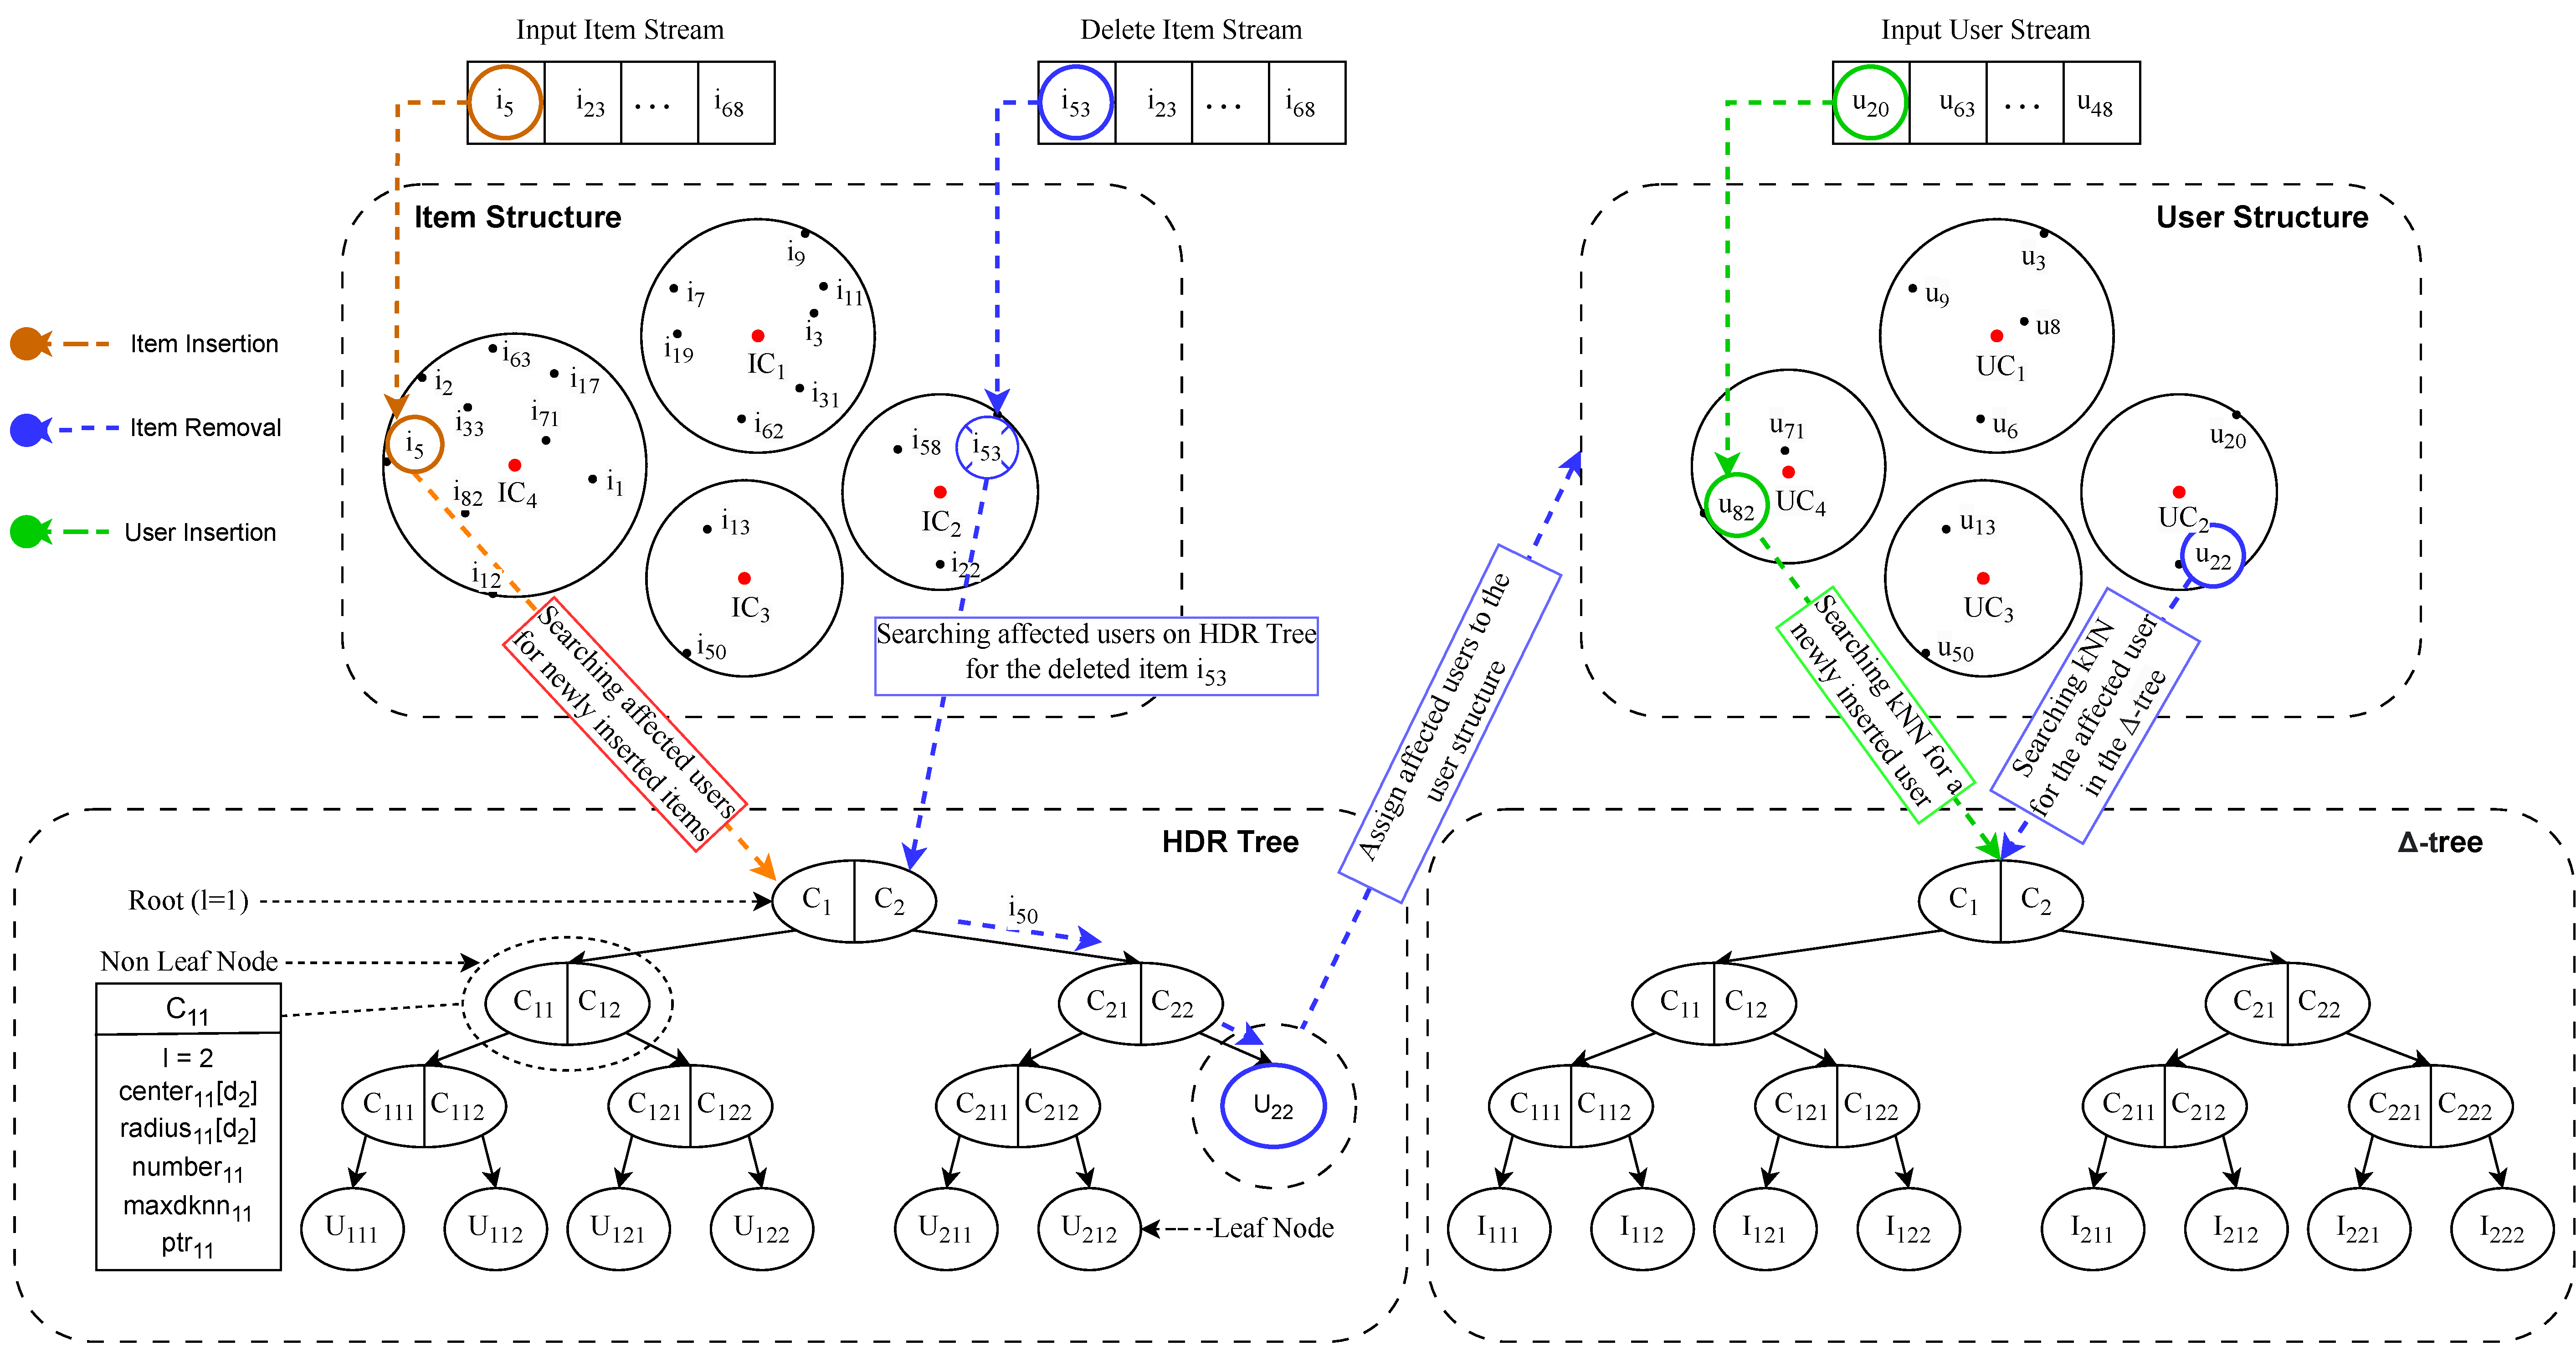
\includegraphics[width=\textwidth]{Images/FDkNNJ.pdf}
    \caption{The general process of cluster-based efficient updating of $KNN_{\bowtie}(U,I)$.}
    \label{fig:cluster_based_update}
\end{figure*}

\subsubsection{Cluster-based efficient updating of $KNN_{\bowtie}(U,I)$ for a batch of inserted points in $U$}

When a batch of data points $u_1, u_2,...u_i,...u_n$ are inserted in $U$, if updating of $KNN_{\bowtie}(U,I)$ is only required to cover the general insertion of points in $U$ but is not for each inserted point, instead of updating $KNN_{\bowtie}(U,I)$ sequentially for each inserted point until gaining the final result, it would be more efficient to calculate the final result of $KNN_{\bowtie}(U,I)$ by first clustering the inserted points into $N$ clusters in the PC space with a specific number $d$ of dimensions then using the cluster-based combined KNN Search algorithm on $\Delta-Tree$ to complete KNN Search for all the points in each cluster at the same time. According to the deduction we have above, if the value $N$ chosen can ensure the points in each cluster get close enough, the searching time for each cluster on the $\Delta-Tree$ can be much shorter than the sum of the time cost for KNN Searching for each point on the $\Delta-Tree$. Therefore, once a appropriate number $N$ of clusters is chosen, the efficiency of calculating the final result of $KNN_{\bowtie}(U,I)$ for a general insertion of points in $U$ by using the strategy of clustering and combined KNN Search for clusters can be much higher than that of the sequential updating strategy. The general process of cluster-based updating of $KNN_{\bowtie}(U,I)$ for a general insertion of points in $U$ is as the green route shows in the Fig.\ref{fig:cluster_based_update}.

\subsubsection{Cluster-based efficient updating of $KNN_{\bowtie}(U,I)$ for a batch of inserted points in $I$}

When a batch of data points $i_1, i_2,...i_j,...i_n$ are inserted in $I$, if updating of $KNN_{\bowtie}(U,I)$ is only required to cover the general insertion of points in $I$ but is not for each inserted point, updating of $KNN_{\bowtie}(U,I)$ can follow the cluster-based schema. Firstly, inserted points can be clustered into $N_0$ clusters in the PC space with a specific number $d_0$ of dimensions. Then for each gained cluster, cluster-based combined RKNN Search algorithm on \hdrtree should be used to complete RKNN Search for all the points in the cluster at the same time. Finally, the KNN Search result of each gained affected point in $U$ should be updated by the newly inserted points in $I$. Such cluster-based updating of $KNN_{\bowtie}(U,I)$ can be much faster than sequential updating once an appropriate number $N_0$ is chosen to let the points in each cluster merge closely. The general process of cluster-based updating of $KNN_{\bowtie}(U,I)$ for a general insertion of points in $I$ is as the red route shows in the Fig.\ref{fig:cluster_based_update}.

\subsubsection{Cluster-based efficient updating of $KNN_{\bowtie}(U,I)$ for a batch of deleted points in $I$}

When a batch of data points $i_1, i_2,...i_j,...i_n$ are deleted from $I$, if updating of $KNN_{\bowtie}(U,I)$ is only required to cover the general deletion of points in $I$ but is not for each deleted point, updating of $KNN_{\bowtie}(U,I)$ can follow the cluster-based schema. Firstly, cluster the deleted points from $I$ into $N_0$ clusters in the PC space with a specific number $d_0$ of dimensions. Then for each gained cluster, implement combined RKNN Search on the \hdrtree to complete RKNN Search for all the points in the cluster at the same time. After that, cluster the gained affected data points in $U$ into $N$ clusters in the PC space with a specific number $d$ of dimensions. Finally, for each of the cluster, apply the combined KNN Search algorithm on the $\Delta-Tree$ to re-compute the KNN members of all the points in the cluster at the same time. If the appropriate numbers of $N_0$ and $N$ can be chosen to ensure tight clusters of deleted points in $I$ and tight clusters of affected points in $U$, cluster-based updating of $KNN_{\bowtie}(U,I)$ can highly outperform sequential updating. The general process of cluster-based updating of $KNN_{\bowtie}(U,I)$ for a general deletion of points in $I$ is as the blue route shows in the Fig.\ref{fig:cluster_based_update}.

\subsubsection{The clustering strategy of cluster-based efficient updating of $KNN_{\bowtie}(U,I)$}

In this paper, before the updating of points in $U$ and $I$ starts, we cluster the initial $U$ into $N$ clusters in the PC space with the number $d$ of dimensions larger than the maximal number of dimensions of the non-leafnodes on the $\Delta-Tree$ and the maximal number of dimensions of the non-leafnodes on the \hdrtree but much smaller than the full number of dimensions of the data points, so that the clusters can keep enough distance information and will not bring heavy cost of distance calculation in the following clustering process for the points need KNN Search after the updating starts. After gaining the clusters, we only record their centers. After the fully dynamic update of $U$ and $I$ starts, When a batch of points in $U$ or being inserted in $U$ needs KNN Search, we cluster them around the centers of the clusters gained from the initial $U$, then for each cluster, the combined KNN Search algorithm can be applied to complete KNN Search for all the points in the cluster at the same time. Such clustering process is on low dimensional PC space, as a result, it may not bring heavy distance calculation cost. And the approach for clustering updated points in $I$ follows the similar schema. 

\begin{comment}
In some cases of practical application of Fully Dynamic KNN Join, focus is only given to calculate the final result of KNN Join for a sequence of updating on $U$ and $I$ while there is no need for the middle states of $KNN_{\bowtie}(U,I)$. For example, lets assume a sequence of updating on $U$ and $I$ that is $\odot_{U}(p_1)$, $\odot_{U}(p_2)$, ...$\odot_{U}(p_i)$...$\odot_{U}(p_n)$, $\odot_{I} (q_1)$, $\odot_{I}(q_2)$...$\odot_{I}(q_j)$...$\odot_{I}(q_m)$, in some cases, we only need to update the final result of $KNN_{\bowtie}(U,I)$ for the whole sequence of updating, but have no need to update $KNN_{\bowtie}(U,I)$ for each $\odot_{U}(p_i)$ and each $\odot_{I}(q_j)$. In the cases discussed above, it would bring redundant computation to sequentially update $KNN_{\bowtie}(U,I)$ because its middle states for each $\odot_{U}(p_i)$ and $\odot_{I}(q_j)$ are not needed. For such scenario only paying attention to the final result of $KNN_{\bowtie}(U,I)$, we introduce an index structure named \todo{need an official name here} $Dual Tree$ \& Clusters for Fully Dynamic KNN Join which supports combined KNN Search for a cluster of $u$ and combined RKNN Search for a cluster of $i$. Based on the novel function of combined search, $Dual Tree$ \& Clusters can improve the efficiency of Fully Dynamic KNN Join by decreasing the calculation for middle states.
\end{comment}

\begin{comment}
For Fully Dynamic KNN Join, there are cases where a batch of same kind updating happens in $U$ or $I$ at the same time and $KNNJ(U,I,k)$ after the batch updating is needed. A batch of same kind updating means a batch insertion of $u$ in $U$ or a batch of deletion of $u$ in $U$ or a batch of insertion of $i$ in $I$ or a batch of deletion of $i$ in $I$. In such cases, it is very costly to calculate $KNNJ(U,I,k)$ after the batch of same kind updating by calculating $KNNJ(U,I,k)$ in all the middle states one by one. For example, lets assume a case where a batch of $u$ that $u_1$, $u_2$, $u_3$......$u_n$ are inserted into $U$ at the same time. Because the insertions are at the same time, only $KNNJ(U,I,k)$ after the batch of insertion is needed. Such result can be calculated by the scheme below. Firstly, regard the batch of insertions at the same time as a sequential process. Then, calculate $KNNJ(U,I,k)$ after the insertion of $u_1$, and calculate $KNNJ(U,I,k)$ after the insertion of $u_1$ and $u_2$......until all the middle states are calculated and $KNNJ(U,I,k)$ after all the insertion is calculated. However, such framework of calculation is too costly because $KNNJ(U,I,k)$ for all the middle states need to be calculated and Search for a single updated point on the index structure (If it is used) needs to be repeated by times equal to the number of the updated vectors. As the best of we know, almost all the existing methods deal with the calculation for $KNNJ(U,I,k)$ after a batch of same kind updating by the awkward framework introduced above. In this part, we will introduce an index structure named HDR Tree \& $\Delta Tree$ \& Clusters for Fully Dynamic KNN Join which supports combined KNN Search for a cluster of $u$ and combined RKNN Search for a cluster of $i$. Based on the novel function of combined search, the newly proposed index structure can improve the efficiency of KNN Join for a batch of same kind updating within Fully Dynamic KNN Join by decreasing the times of calculation of the middle states.   
\end{comment}

\begin{comment}
\subsubsection{The Structure of $Dual Tree$ \& Clusters}
The structure of $Dual Tree$ \& Clusters consists a HDR Tree, a $\Delta$ Tree, a set $Su$ of clusters $Cu$ of $u$ and a set $Si$ of clusters $Ci$ of $i$. Each $Cu$ contains the following attribute: a list $U_{Cu}$ of its members, its radius and center in a $d_{Cu}-$ dimensional PC space ($d_{Cu}$ is no smaller than the maximal dimension number of the non-leafnodes on the $\Delta$ Tree, so that $dist_{d(l(C))}(center_{d_{Cu}}(Cu), C)$ is available for every cluster $C$ on the $\Delta$ Tree, all the clusters in $Su$ share the same $d_{Cu}$), and a list $L_{dist}(Cu)$ that contains $dist_{d(l(C_{ij}))}(center_{d_{Cu}}(Cu),center_{d(l(C_{ij}))}(C_{ij}))$ for each $C_{ij}$ ($i=1,2,3...L_{\Delta}, j=1,2,3...num(i)$) on the $\Delta$ Tree. And $Ci$ is the mirrored version of $C_u$, that contains the following features: a list $I_{Ci}$ of its member, its radius and its center in a $d_{Ci}$ dimensional PC space ($d_{Ci}$ is no smaller than the maximal number of dimensions of the non-leafnodes on the HDR Tree, all the clusters in $Si$ share the same $d_{ci}$), and a list $L_{dist}(Ci)$ that contains $dist_{d(l(C_{ij}))}(center_{d_{Ci}}(Ci), center_{d(l(C_{ij}))}(C_{ij}))$ for each $C_{ij}$ ($i=1,2,3...L_{\Delta}, j=1,2,3...num(i)$) on the $\Delta$ Tree. The table-2 show the attributes of $Cu$ and $Ci$. 

The numbers of clusters in $Su$ and $Si$ are specified by the users. The center of each $Cu$ and the center of each $Ci$ are initialized based on the initial state of $U$ and $I$. The data points in $U$ on the initial stage would be projected into a $d_{Cu}$-dimensional PC space, then, $k-means$ would be performed on the low-dimensional versions of the points in $U$, finally, the center of $d_{Cu}$-dimensional of each produced cluster by $k-means$ would be applied as the center of each $Cu$.  Initialization of the center of each $Ci$ is the mirrored version of that for $Cu$, so we skip it here. In the process of FDKNNJ, we do not change the center of $Cu$ and $Ci$. After the centers of the clusters are initialized, we calculate the distance from the center of each $Cu$ to the center of each $C_{ij}$ of $d(l(C_{i,j}))$-dimensional on the $Delta$ Tree, and store the distance values in $L_{dist}(Cu)$. And we calculate the distance from the center of each $Ci$ to the center of each $C_{ij}$ of $d(l(C_{i,j}))$-dimensional on the HDR Tree, and store the distance values in $L_{dist}(Ci)$. Below we will introduce the efficient strategy of updating the final result of $KNN_{\bowtie}(U,I)$ for a sequence of same kind updating on $U$ or $I$.

\begin{table}[t]
    \begin{minipage}{.45\linewidth}
        \centering
        \footnotesize
        \caption{\footnotesize Attributes of $Cu$.}
        \label{tab:symbol_cu}
        \begin{tabular}{|c|p{0.62\linewidth}|}
            \hline
            $U_{Cu}$\\
            \hline
            $center_{d_{cu}}(Cu)$\\
            \hline
            $r_{d_{cu}}(Cu)$\\
            \hline
            $L_{dist}(Cu)$\\
            \hline
        \end{tabular}
    \end{minipage}%
    \hspace{0.1\linewidth}% Adjust the space between tables
    \begin{minipage}{.45\linewidth}
        \centering
        \footnotesize
        \caption{\footnotesize Attributes of $Ci$.}
        \label{tab:symbol_ci}
        \begin{tabular}{|c|p{0.62\linewidth}|}
            \hline
            $U_{Ci}$\\
            \hline
            $center_{d_{ci}}(Ci)$\\
            \hline
            $r_{d_{ci}}(Ci)$\\
            \hline
            $L_{dist}(Ci)$\\
            \hline
        \end{tabular}
    \end{minipage}
\end{table}
\end{comment}

\begin{comment}
\begin{table}[t]
\footnotesize
\caption{\footnotesize Attributes of $Cu$.}
\label{tab:symbol}
\centering
\begin{tabular}{|c|p{0.62\linewidth}|}
\hline

\hline
$U_{Cu}$\\
\hline
$center_{d_{cu}}(Cu)$\\
\hline
$r_{d_{cu}}(Cu)$\\
\hline
$L_{dist}(Cu)$\\
\hline
\end{tabular}
\end{table}

\begin{table}[t]
\footnotesize
\caption{\footnotesize Attributes of $Ci$.}
\label{tab:symbol}
\centering
\begin{tabular}{|c|p{0.62\linewidth}|}
\hline

\hline
$U_{Ci}$\\
\hline
$center_{d_{ci}}(Ci)$\\
\hline
$r_{d_{ci}}(Ci)$\\
\hline
$L_{dist}(Ci)$\\
\hline
\end{tabular}
\end{table}

\todo{Hi, nimish, could you please help me move the table 3 to the left side of table 2? Thank you so much! }
\end{comment}

\begin{comment}
\begin{figure*}[ht]
    \centering
    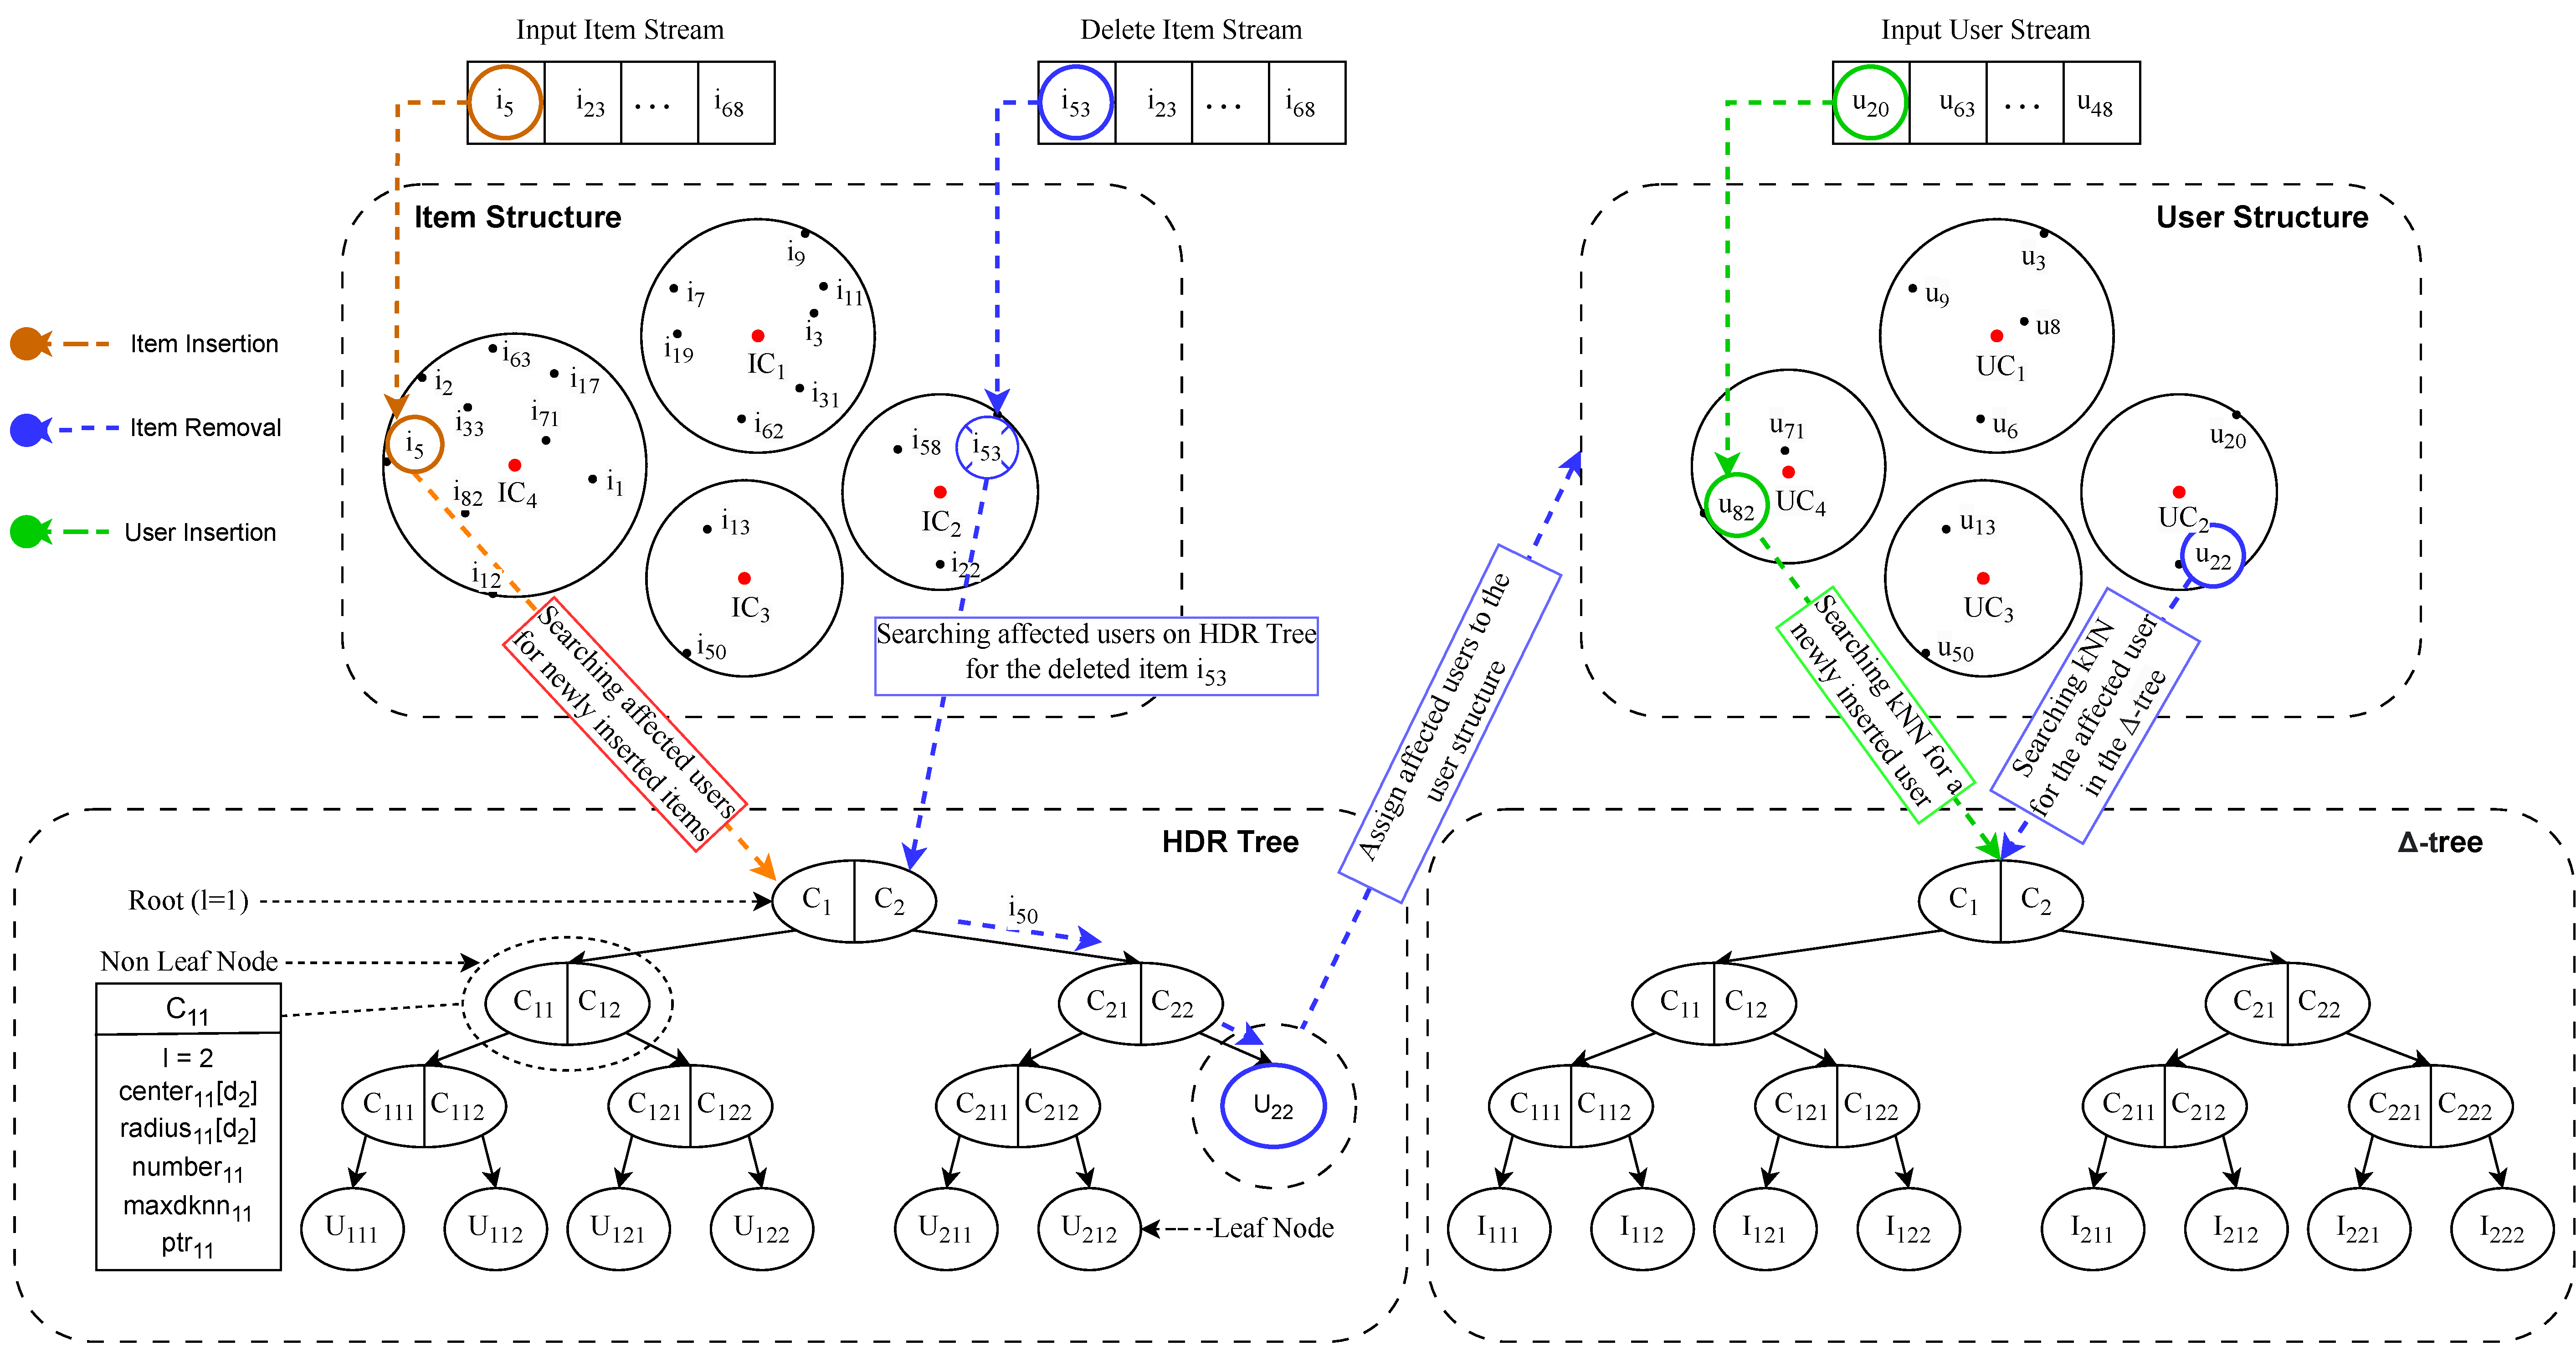
\includegraphics[width=\textwidth]{Images/FDkNNJ.pdf}
    \caption{An example performing a fully dynamic kNN join operation with f=2, which involved answer (i.e., item data point) insertion, answer removal and query insertion.}
    \label{fig:fdknnj-user-insertion}
\end{figure*}

\subsubsection{Efficiently Updating $KNN_{\bowtie}(U,I)$ for a sequence of $\oplus_{i}I$}
In this part, we will introduce an efficient algorithm to calculate the final result of $KNN_{\bowtie}(U,I)$ for a sequence of $\oplus_{i}I$ rather than sequential calculation for every $\oplus_{i}I$. This algorithm takes the set named $set(i)$ of $i$ inserted in $I$ as its parameter.

\begin{algorithm}
\caption{UpdateKNN$_{\bowtie}$\_I\_efficient($set(i)$,$insert$)}\label{alg:updateknn_I_efficient}
\KwData{a set of $i$ inserted in $I$}
\KwResult{The final result of $KNN_{\bowtie}(U,I)$ for the insertion of $set(i)$ in $I$}
\For{$i$ in $set(i)$}{
  $C$=$argmin(dist_{d(Ci)}(center_{d(Ci)}(Ci), i))$;
  $C.push(i)$;
  $Update_\Delta_Insert(i, root_{\Delta})$
}
\For{$Ci$ in $Su$}{
  calculate $r_{d_{Ci}}(Ci)$;
}
\For{$Ci$ in $Si$}{
  RKNNSearch_update_cluster($root_{HDR}$, $Ci$);
  Adjust maxdknn values for HDR Tree;
  $Ci.clear()$;
}
\end{algorithm}


\begin{algorithm}
\caption{UpdateKNN$_{\bowtie}$\_I\_efficient($set(i)$,$delete$)}\label{alg:updateknn_I_efficient_delete}
\KwData{a set of $i$ deleted in $I$}
\KwResult{The final result of $KNN_{\bowtie}(U,I)$ for the deletion of $set(i)$ in $I$}
\For{$i$ in $set(i)$}{
  $C$=$argmin(dist_{d(Ci)}(center_{d(Ci)}(Ci), i))$;
  $C.push(i)$;
  $Update_\Delta_Delete(i, root_{\Delta})$
}
\For{$Ci$ in $Si$}{
  calculate $r_{d_{Ci}}(Ci)$;
}
\For{$Cu$ in $Su$}{
  RKNNSearch_delete_cluster($root_{HDR}$, $Ci$);
  $Ci.clear()$;
}
\For{$u$ in $R_p$}{
  $C$=$argmin(dist_{d(Cu)}(center_{d(Cu)}(Cu), u))$;
  $C.push(u)$;
}
\For{$Cu$ in $Su$}{
  calculate $r_{d_{Cu}}(Cu)$;
}
\For{$Cu$ in $Su$}{
  Combined_KNNSearch($root_{\Delta}$, $Cu$);
  $Cu.clear()$;
}
Adjust maxdknn values for HDR Tree;
\end{algorithm}

\begin{algorithm}
\caption{UpdateKNN$_{\bowtie}$\_U\_efficient($set(u)$,$insert$)}\label{alg:updateknn_U_efficient_insert}
\KwData{a set of $u$ inserted in $I$}
\KwResult{The final result of $KNN_{\bowtie}(U,I)$ for the insertion of $set(u)$ in $U$}
\For{$U$ in $set(u)$}{
  $C$=$argmin(dist_{d(Cu)}(center_{d(Cu)}(Cu), u))$;
  $C.push(u)$;
  $Update_HDR_Insert(u, root_{HDR})$
}
\For{$Ci$ in $Si$}{
  calculate $r_{d_{Ci}}(Ci)$;
}
\For{$Cu$ in $Su$}{
  Combined_KNNSearch($root_{HDR}$, $Cu$);
  $Cu.clear()$;
}
Adjust maxdknn values for HDR Tree;
\end{algorithm}

\begin{algorithm}
\caption{RKNNSearch_update_cluster($node$, $Ci$)}\label{alg:RKNN Search}
\KwData{a node $node$ on the HDR Tree, the cluster $Ci$ of inserted $i$}
\KwResult{The affected set $R_p$ of $u$ which is a sub set of $U$, and the updated KNN members of $u$ in $R_p$}

\eIf{$node$ is a $LN$}{
    \For{each $u$ in $node$}{
      \If{$dist_{d_{Ci}}(u, center_{d_{Ci}}(Ci))-r_{d(Ci)}(Ci)<dknn(u)$}{
        \For{each $i$ in $Ci$}{
          \If{$dist(i,u)\leq u.dknn$}{
              delete $i_furthest$ from $KNN(u,I)$;\\
              push $i$ into $KNN(u,I)$;\\
              update $dknn(u)$;\\
          }
        }  
      }  
    }
}
{
$C_p = NLN.clusters$;\\
\For{each clusters $C : C_p$}{
    \If{$dist_{d(l(C))}(center_{d(l(C))}(C), center_{d_{Ci}}(Ci)) - r_{d(l(C))}(C)- r_{d(Cu)}(Cu)<maxdknn(C)$}{
        RKNNSearch_update_cluster $(node.children[j],$Ci$);$
    }
}
}
\end{algorithm}
\end{comment}